	\documentclass[
	  paper    = a4,
	  BCOR     = 10mm,
	  twoside,
	  fontsize = 12pt,
	  fleqn,
	  toc      = bibnumbered,
	  toc      = listofnumbered,
	  numbers  = noendperiod,
	  headings = normal,
	  listof   = leveldown,
	  version  = 3.03
	]{scrreprt}

	\usepackage[utf8]{inputenc}
	\usepackage[T1]{fontenc}
	\usepackage{color}
	\usepackage{amsmath}
	\usepackage{graphicx}
	\usepackage[english]{babel}
	% \usepackage{natbib}

	% \usepackage[pagebackref=true,breaklinks=true,letterpaper=true,colorlinks,bookmarks=false]{hyperref}
	\usepackage[pagebackref=true,breaklinks=true,colorlinks,bookmarks=false]{hyperref}
	\usepackage{csquotes}
	\usepackage{times}
	\usepackage{epsfig}
	\usepackage{graphicx}
	\usepackage{amsmath}
	\usepackage{dsfont}
	\usepackage{amssymb}
	\usepackage{mathtools}
	\usepackage{caption}
	\usepackage{float}
	\usepackage{subcaption}
	\usepackage{xspace}
	\usepackage{tikz}
	\usetikzlibrary{bayesnet}
	% \usepackage{comment}
	\usepackage{xcolor}
	\newcommand\todo[1]{\textcolor{red}{#1}}
	\renewcommand\todo[1]{}

	\newcommand\expr[1]{\textcolor{red}{#1}}
	\renewcommand\expr[1]{}

	\newcommand\note[1]{\textcolor{blue}{#1}}
	\renewcommand\note[1]{}

	\definecolor{darkblue}{rgb}{0.0,0.0,0.4}
	\definecolor{darkgreen}{rgb}{0.0,0.4,0.0}
	\hypersetup{%
	    colorlinks,
	    linkcolor=black,
	    citecolor=darkgreen,
	    urlcolor=darkblue
	}

	\makeatletter
		\DeclareRobustCommand\onedot{\futurelet\@let@token\@onedot}
		\def\@onedot{\ifx\@let@token.\else.\null\fi\xspace}
		\def\eg{\emph{e.g}\onedot} \def\Eg{\emph{E.g}\onedot}
		\def\ie{\emph{i.e}\onedot} \def\Ie{\emph{I.e}\onedot}
		\def\cf{\emph{c.f}\onedot} \def\Cf{\emph{C.f}\onedot}
		\def\etc{\emph{etc}\onedot} \def\vs{\emph{vs}\onedot}
		\def\wrt{w.r.t\onedot} \def\dof{d.o.f\onedot}
		\def\etal{\emph{et al}\onedot}
	\makeatother

\begin{document}
	% %% Titelseiten ähnlich zum Layout des Formulars von der
%% Fakultät für Physik und Astronomie
%%
%% Weitere Infos:
%% http://www.physik.uni-heidelberg.de/aktuelles/studium/
%% (PDF link: ...studium/download/145/Vorlage_Diplomarbeit_Formular.pdf)

%% Titelintro
\thispagestyle{empty}
\begin{center}
  \renewcommand{\baselinestretch}{2.00}
  \Large\sffamily
  Fakult\"{a}t f\"{u}r Physik und Astronomie\\
  \large
  Ruprecht-Karls-Universit\"{a}t Heidelberg
  \par\vfill\normalfont
  Masterarbeit\\
  Im Studiengang Physik\\
  vorgelegt von\\
  (Vor- und Zuname)\\
  geboren in (Geburtsort)\\
  (Jahr der Abgabe)\\
\end{center}
\newpage

%% Titelseite
\thispagestyle{empty}
\begin{center}
  \renewcommand{\baselinestretch}{2.00}
  \Large\bfseries\sffamily
    (Titel)\\
    (der)\\
    (Masterarbeit)
  \par
  \vfill
  \large\normalfont
  Die Masterarbeit wurde von (Vorname Name)\\
  ausgef\"{u}hrt am\\
  (Institut)\\
  unter der Betreuung von\\
  (Frau/Herrn Prof./Priv.-Doz. Vorname Name)
  %% Bei externen Masterarbeiten hier noch den zweiten Betreuer einfügen
  %% und den vspace in Z. 45 entsprechend reduzieren
\end{center}\par
\vspace{5\baselineskip}

% Zeilenabstand zurücksetzen
\renewcommand{\baselinestretch}{1.00}\normalsize % select either german
	% %% this will generate title pages similar to the template provided
%% by the Department of Physics and Astronomy Heidelberg
%%
%% More information:
%% http://www.physik.uni-heidelberg.de/aktuelles/studium/
%% (PDF link: ...studium/download/145/Vorlage_Diplomarbeit_Formular.pdf)

%% Titleintro
\thispagestyle{empty}
\begin{center}
  \renewcommand{\baselinestretch}{2.00}
  \Large\sffamily
  Department of Physics and Astronomy\\
  \large University of Heidelberg
  \par\vfill\normalfont
  Master thesis\\
  in Physics\\
  submitted by\\
  (name and surname)\\
  born in (place of birth)\\
  (year of submission)
\end{center}
\newpage

%% Titlepage
\thispagestyle{empty}
\begin{center}
  \renewcommand{\baselinestretch}{2.00}
  \Large\bfseries\sffamily
    (Title)\\
    (of)\\
    (Master thesis)
  \par
  \vfill
  \large\normalfont
  This Master thesis has been carried out by (Name Surname)\\
  at the\\
  (institute)\\
  under the supervision of\\
  (Frau/Herrn Prof./Priv.-Doz. Name Surname)
  %% additionally insert second supervisor here if carrying out an
  %% external diploma thesis. Reduce vspace in L. 44 accordingly.
\end{center}\par
\vspace{5\baselineskip}

% reset baselinestretch
\renewcommand{\baselinestretch}{1.00}\normalsize % or english title page
	% %% Abstract page
%% =============
%%
%% Content of abstract pages has been put into seperate pages to simplify
%% word counting. Use e.g. the unix command
%%   wc abstract-ger.tex
%% or
%%   wc abstract-eng.tex
%% to get the number of words contained in these files.
\thispagestyle{empty}
\begin{center}
  \begin{minipage}[c][0.48\textheight][b]{0.9\textwidth}
    \small
    \textbf{
      (Titel der Masterarbeit - deutsch):
    }\par
    \vspace{\baselineskip}
    Objektrepräsentationen sind von fundamentaler Bedeutung für viele Anwendungen in Computer Vision. Die vorliegende Arbeit präsentiert und evaluiert einen unüberwachten Ansatz, um eine kompositionelle Teilrepräsentation von Objekten zu lernen, welche die geometrische Form und die visuelle Erscheinung für jeden Objektteil trennt. Um die Faktoren von Form und Erscheinung zu trennen, wird Invarianz unter Transformationen des jeweils anderen Faktors angenommen. Zusätzlich wird verwendet, dass räumliche Form equivariant bezüglich räumlicher Transformationen ist. Diese Annahmen werden in eine Autoencoder Architektur eingebaut, die so konstruiert ist, dass eine lokale Interpretation der Objektteile gewahrt bleibt. \\
Die Methode weist dem Objekt Teile zu, die das Objekt konsistent und sinnvoll abdecken, ohne manuelle Überwachung oder a priori Annahmen über die Objektklasse zu benötigen.
Die Methode wird evaluiert auf einer Anzahl an herausfordernden Datensätzen, wobei die Objektklassen variieren: von menschlichen Gesichtern über menschliche Personen bis hin zu Hunden, Katzen und Vögeln. Das unüberwachte Lernen von Form wird evaluiert, indem aus den entdeckten Teilen, Objektmarkierungen regressiert werden. Der neueste Stand der Forschung wird hierbei signifikant geschlagen. Darüber hinaus wird gezeigt, dass die Repräsentation tatsächlich in Form und Erscheinung aufspaltet und lokale Teile unabhängig voneinander lernt.

  \end{minipage}\par
  \vfill
  \begin{minipage}[c][0.48\textheight][b]{0.9\textwidth}
    \small
    \textbf{
      (Title of Master thesis - english):
    }\par
    \vspace{\baselineskip}
    %% Latex markup and citations may be used here
  Object representations are of paramount importance for various computer vision applications. %Learning such a      model without supervision is still an open challenge. %Frequently used holistic object representations limit a     deep understanding of its spatial structure.
  The thesis at hand presents an unsupervised approach to learn a part representation of an object, disentangling the factors of geometric shape and visual appearance for each part. %The invariance of one factor when        the other is transformed in a two-stream auto-encoding framework.
  To disentangle, each shape is assumed to be invariant under transformations of appearance and vice versa. Additionally, shape is assumed to be equivariant with respect to spatial transformations. These assumptions are implemented in a two-stream autoencoding framework for detecting parts, while the architecture is designed to maintain the local nature of the parts.\\
  %We derive explicit invariance and equivariance constraints for such a decomposition and implement these in a      generative framework. % by our shape representation.
  Trained without any manual supervision or prior information on the object class, the model learns to discover parts, that cover the whole object consistently. We evaluate this on a diverse selection of challenging datasets, the object classes ranging from human faces and bodies to dogs, cats and birds.
  State-of-the-art methods are significantly outperformed in terms of unsupervised landmark regression.
  % The margin is especially large on datasets with strong articulation.
  Additionally, we show that our model actually learns to disentangle shape from appearance and learns local parts independently.
 %Unsupervised results for datasets with background clutter and significant articulation have never been            obtained before.

% To show that the disentanglement is indeed achieved, we evaluate the disentanglement performance against a shape-supervised state-of-the-art disentanglement method and perform favorably (Chapter~\ref{sec:disentangling}).
% \item \textit{Hypothesis \emph{ii)}: Learning unsupervised disentanglement without any assumptions is fundamentally impossible. In accordance with the literature on causal learning \cite{pearl18impediments}, disentangling causal factors requires model assumptions and/or interactional data - instead of observational (raw) data.}


	% To address these hypotheses, we \textit{explain}, \textit{validate} and \textit{evaluate} a method for unsupervised shape learning: \textit{Unsupervised Part-wise Disentanglement of Shape and Appearance} developed by Lorenz \etal\ 2018\todo{cite properly}.
%
%
	% To \textit{explain}, after theoretical prerequisites (Chapter~\ref{sec:prerequisites}) we give an overview over state-of-the-art unsupervised disentangling literature and situate the proposed method in relation to the literature (Chapter~\ref{sec:literature}). In particular, we carve out the necessary aspects of an approach for disentangling causal factors and analyze the current state of research in order to indicate future directions.\todo{do that for real!}
	% We subsequently disclose our method (Chapter~\ref{sec:method}).
%
%
	% To \textit{validate}, we show that the proposed method outperforms the state-of-the-art for unsupervised learning of object shape on miscellaneous datasets, featuring human and animal faces and bodies (Chapter~\ref{sec:shapelearning}).
	% We also contribute several self-made video datasets for disentangling human pose from appearance, for articulated animal motion and for articulated composite objects. We highlight the specific challenges of these datasets and elucidate how the proposed method tackles them.
%
%
	% To \textit{evaluate}, we perform ablation studies on critical components of the method. In addition, we compare to a part-wise shape learning method which does make the goal of disentangling explicit.
%
%
	% % In short, our results are a big improvement upon the state-of-the-art in unsupervised object shape learning. This confirms the first hypothesis. To complement the learned shape in a generative process, object appearance is disentangled from shape. The achieved disentanglement with our causal assumptions, and the not-achieved disentanglement when dropping these assumptions, confirms the second hypothesis.

  \end{minipage}
\end{center}


	\tableofcontents
	\newpage

	%&tex
\chapter{Introduction}
	Computer vision is the scientific endeavour to algorithmically understand patterns in images.
	Structures and processes in the physical world interact in complex ways to generate an image. The image then acts as a mirror, in which these elements of the world are reflected and leave patterns.
	To recognize patterns in an image, means in essence, to use this mirror as a window to observe the reality lurking behind it, \ie to measure the causal elements that contributed to the image generation.
	Typically, objects appear in an intricated interaction of many factors of variation.
	For example, given the object class of people, persons can vary in their visual appearance by clothing and skin color or in their geometric structure due to their pose or body physique. \note{The image generation itself may further add factors like illumination, viewpoint or contrast.}
	For articulated object classes the most prominent factors of variation are geometric shape and visual appearance\todo{ (add reference here?)}.
	Disentangling these factors is a difficult problem, due to the intricated interplay of shape and appearance, especially under heavy articulation.
	The complexity enters, as a variation in shape is a change of the images domain rather than a change of its values~\cite{shu18shapeappear}.
	Consider a person raising his arm: the color and texture of his pullover sleeve intrinsically does not change, but appears at a different location in the image. An efficient model for shape should cover all possible states of the object and preserve the local linkage to its intrinsic appearance.

\section{Why Disentangle Causal Factors?}
	\note{Above, we framed disentangling generative factors as a scientific measurement process. An interaction of physical elements in the world is captured in an image, which can be treated as a scientific measurement of reality. Discerning patterns, and disentangling sources of patterns from each other, will then be defined as \textit{understanding} the world. What can be gained from such an \textit{understanding}?}
	On the one hand, there are pragmatic reasons to aim at extracting disentangled factors from images: to successfully transfer a representation between different tasks, typically only a few factors are relevant \cite{bengio13rep}.
	Efficient transfer and multi-task learning should account for this.
	On the other hand, learning to capture external mechanisms in appropriate internal representations, can be seen as a step to automate visual reasoning itself.
	Once disentangled, a factor can be manipulated individually to make a targeted change in an image. Thereby, humans may change images at will, but also machines may reason about the world \cite{pearl18impediments}, by simulating changes to factors internally in their model of the world.
	Thought experiments like \textit{"imagine, how ridiculous you would look, if you wore that hot pants"} are manageable tasks for the human imagination, but are out of the league for currently used generative image models \cite{goodfellow14gan, kingma13vae}, that typically rely on non-interpretable vector spaces with entangled dimensions.
	Building imagination machines has been proposed as a goal for artificial intelligence research recently \cite{mahadevan18imagine}.
	% To imagine, is to manipulate of an internal model to generate internal images.
	In this sense, in the context of generative modelling, disentangling factors could as well lead the way from a science of images to a science of imagination.
	% \note{Data-driven algorithms for pattern recognition good recently}
	% \note{how much and how to incorporate prior knowledge}
	% \note{is this necessary, theoretical arguments against}
	% \begin{itemize}
		% \item Computer vision: automatically discern patterns, that reflect structures in physical world
		% \item Why disentangle: detect causal factors to image
		% \item Pragmatic reason: efficient transfer learning, multi-task learning
		% \item Philosophical reason: build machines that understand mechanisms, reason about world \cite{Pearl:2018im}
		% \item Targeted changes $\rightarrow$ thought experiments; not possible for e.g. GAN, VAE\ \textit{"imagine, ..."}\ science of images $\Rightarrow$ science of imagination \cite{Mahadevan:2018tz}.
	% \end{itemize}

\section{How not to Disentangle.}
	\begin{figure}[t]
		\centering
		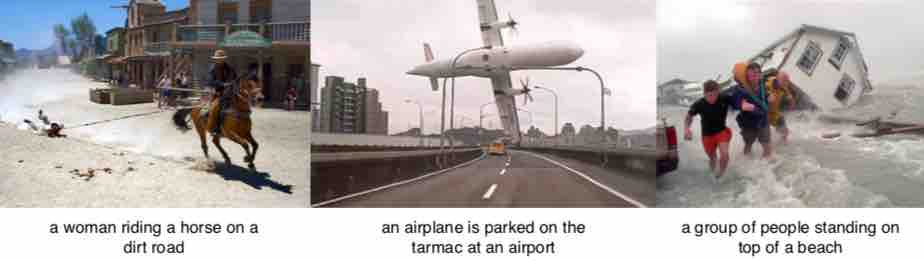
\includegraphics[trim={0cm 0cm 0cm 0cm},clip, width=1.\linewidth]{fig/notcausal}
		\caption{The image captions are generated by a deep neural network (Neuraltalk2) \cite{karpathy15neuraltalk}. Yet, common sense understanding of psychological and physical entities in terms of causal relationships and narratives is absent \cite{tenenbaum18think}. Instead, the neural network seems to capture mere associations.}
		\label{fig:notcausal}
	\end{figure}
	Can machines tell a story? Carefully observe your own mind, when viewing the images shown in Fig. \ref{fig:notcausal}: observe how the human mind immediately interprets and jumps to conclusions, tries to tell itself a story that explains an image, whereas the machine (in this case, NeuralTalk2 \cite{karpathy15neuraltalk}), is comically descriptive in contrast.
	The missing \textit{common sense} may be due to a missing causal reasoning, due to a missing disentangled causal representation of the world.
	But how to learn a disentangled representation from scratch, \ie from raw image data?
	As we will find out \todo{ref to sec}, disentangling causal factors from raw image data, without any side information is impossible theoretically, and can only work based on statistical assumptions.
	Lets consider an example:
	Given an image dataset of human persons, that has strong variation in the pose and in the appearance of the persons, how to find these two underlying axes of variation (pose and appearance)? Lets suppose the distribution of variation follows a two-dimensional Gaussian distribution, one dimension for pose, one for appearance. The learning algorithm has access to randomly sampled images from this distribution. An intelligent data compression algorithm will be able to fit a function from the images to the two-dimensional subspace, which explains (by assumption in this example) the variation in the dataset.
	But are the two dimensions, that the algorithms finds disentangled? No. In fact, any linear combination of pose and appearance and its orthogonal complement are equally valid to span the subspace of underlying variation. Just from observing a two-dimensional Gaussian, no meaning will be attached to the axes. In practice, this problem is often circumvented by first fitting a generative model to the image dataset and \textit{afterwards} interpolating in the latent space to determine (by human judgement) the axes of interest (here the pose or appearance axis). The meaning of pose and appearance as independent factors comes from the fact, that it is easily possible in the real world to change one factor without the other. A person moving without loosing clothes is a trivial example for that.
	In summary, on the basis of dataset statistics one cannot disentangle causal factors, if the information about how to select the axes, \ie which factors to separate, is not contained in the raw data.
	Fitting a model to the data distribution, does in general not give insight into how the data was generated.

\section{How can Humans Disentangle?}
% \section{What can Machine Learning Learn from Humans?}
	The dichotomy between humans and machines is constructed, of course, since on a fundamental level humans are machines.
	\note{explain and state performance gap in lacking reasoning, causal discovery, }
	But in this context, the distinction between humans and machines shall refer to the current gap between human and machine learning performance, in terms of inferring generative factors and reasoning (again, cf. Fig. \ref{fig:notcausal}).
	So, what advantageous characteristics does the human mind have, that are lacking in data-driven machine learning algorithms?

	\emph{Priors.}
		Whether acquired or inherited, certain inductive priors seem to guide the human learning in its early phases \cite{tenenbaum18think}.
		Archetypal knowledge of psychology \cite{jung68archetype}, a universal grammar for language \cite{chomsky00horizons} and causal intuitions on everyday physics \cite{teglas11intuitive} are some of the cognitive priors, that could explain the intuitive psychology, the rapid language acquisition and the remarkable causal inference from limited amount of data.

	\emph{Data.}
		Not only quantity, but also quality of data. Machine learning on images is commonly posed as the task to learn from randomly sampled images from a data set. But humans do not perceive the world in arbitrary samples.
		To humans, the world appears in a temporal sequence, which reveals how generative factors change and persevere across time. Instead of focusing on datasets with static images, sampled at random so that the images may have nothing to do with each other, algorithms should use video datasets and harness the rich temporal information.\\
		Another key difference is, that humans interact with their environment.
		That means, humans know change, not only by observing change (as in a temporal sequence), but also by changing.
		Anyone, who has watched a human infant play, can affirm that the learning mind is obsessed with interaction and change. The inevitable destruction around a young human is no accident, but a result of curious learning.
		\note{Whether consciously by performing controlled experiments or by subconscious cues \cite{wall08egomotion}:}
		\textit{Interaction is crucial for a learning mind.}

		% causal inference
		% 3. Learning by interacting: knowing change by changing.
		% second rung on causal ladder (Pearl): intervention. (, acting) What happens if I do?
		% P(s, do(a))
		% Others: counterfactual (imagining), association.
		% In humans e.g. egomotion cues: how does image on retina change if I move.

	\emph{Models.}
	% humans what model: imagination: e.g.
		Humans are able to imagine. That presupposes an internal model of the world, to which specific changes of representational factors can be applied.
		% So-called dreaming neural networks can distract from the fact that human imagination is make changes to the world that it did not observe.
		In machine learning, fitting neural network models as functions to approximate datasets has seen tremendous progress recently, to the point, that it is considered a solved problem \todo{cite something, maybe bigGAN etc)}. This progress is mainly due to the effectiveness of neural networks to fit high-dimensional functions. But a probabilistic fit to a dataset, however complex and rich, is not a causal model. Even if one were to obtain a probabilistic model over all images the world (one could start with \eg ImageNet \cite{russakovsky15imagenet}), this would tell very little about the real-world (causal) relationships between objects.
		\note{One could hope for relationships to emerge by data compression alone, but }
		\note{A step towards intelligence would be to automate the finding of "meaning" in the learned latent spaces. But meaning has to come from somewhere, and will not emerge from the data itself.}

	What can we learn from these differences? An algorithm to understand the world: should contain useful \textit{prior} assumptions to efficiently use \textit{data} that contains the necessary causal relationships and interactions, to learn a useful \textit{model} of the world.

% \section{How to Disentangle?}
	% change factor $\rightarrow$  image change equivariantly, leave others invariant
	% $\rightarrow$  equivariance, invariance
%
	% change can be mimicked artificially
	% Intelligent pattern recognition algorithms, fuelled by sensory data as learning material alone, may ultimately drive the way to a full-blown artificial intelligence, reasoning about the world on its own. - That is the reasoning behind data-driven and assumptionless machine learning approaches that have conquered several research communities.
	% A theoretical objection to driving-only-with-data comes from the causal literature: For an understanding of the world, an algorithm needs to model causal processes, that cause an image to be generated.

\section{Contributions}
	This thesis makes two theses:
	\begin{itemize}
		\item  \textit{Hypothesis \emph{i)}: Unsupervised learning of object shape benefits from abstracting away the shapes complement, namely the object appearance. Explaining away the appearance factor can be achieved by a disentangled generative modelling of both factors.}
		\item \textit{Hypothesis \emph{ii)}: Learning unsupervised disentanglement without any assumptions is fundamentally impossible. In accordance with the literature on causal learning \cite{pearl18impediments}, disentangling causal factors requires model assumptions and/or interactional data - instead of observational (raw) data.}
	\end{itemize}
	% \emph{ii)} Following the need to interact with the world, need to change, need to model physical reality -> image transformations, analyis-by-synthesis}
	To address these hypotheses, we \textit{explain}, \textit{validate} and \textit{evaluate} a method for unsupervised shape learning: \textit{Unsupervised Part-wise Disentanglement of Shape and Appearance} developed by Lorenz \etal\ 2018\todo{cite properly}.


	To \textit{explain}, we give an overview over state-of-the-art unsupervised disentangling literature and situate the proposed method in relation to the literature. In particular, we carve out the necessary aspects of an approach for disentangling causal factors and analyze the current state of research in order to indicate future directions.


	To \textit{validate}, we show that the proposed method outperforms the state-of-the-art for unsupervised learning of object shape on miscellaneous datasets, featuring human and animal faces and bodies.
	We also contribute several self-made video datasets for disentangling human pose from appearance, for articulated animal motion and for articulated composite objects. We highlight the specific challenges of these datasets and elucidate how the proposed method tackles them.


	To \textit{evaluate}, we perform ablation studies on critical components of the method. In addition, we compare to a part-wise shape learning method which does make the goal of disentangling explicit.
	To show that the disentanglement is indeed achieved, we evaluate the disentanglement performance against a shape-supervised state-of-the-art disentanglement method and perform favorably.


	In short, our results are a big improvement upon the state-of-the-art in unsupervised object shape learning. This confirms the first hypothesis. To complement the learned shape in a generative process, object appearance is disentangled from shape. The achieved disentanglement with our causal assumptions, and the not-achieved disentanglement when dropping these assumptions, confirms the second hypothesis.

	%&tex
\chapter{Prerequisites on Learning Disentanglement}\label{sec:prerequisites}

\section{Learning from Data}
	{Learning from data} is commonly understood as the ability of algorithms to improve their performance on a task with experience accumulated from the observation of data \cite{goodfellow16dlb}. The source of data is usually a dataset - set of data points $X = \{x_i | i \in \{1\ldots n\} \}$, which are sampled from a probability distribution $x_i \sim p(x)$.
	In general, these data points are multi-dimensional. In computer vision in particular, data are images $\mathbf{x}$ with height $h$ and width $w$, so that the data points are $\mathbf{x} \in \mathbb{R}^{h \times w}$.

	\subsection{Supervised}\label{sec:supervised}
		The term {supervised learning} denotes the task to learn a mapping from data points $x_i$ to target labels $y_i$.
		A supervised algorithm has access to data-label pairs  $(y_i, x_i) \sim p(y, x)$, in order to estimate the connection between data points and labels, either in form of a conditional probability $p(y|x)$, or in form of a deterministic function $y = f(x)$.
		The label $y$ can be either discrete (\eg information about an object class) or continuous (\eg the location of an object part in an image).
		Recent advances, in particular the effectiveness of neural network models (cf. Sec. \ref{sec:neuralnetworks}) on big datasets, have led to huge progress on problems that can be formulated as regression or classification. That is why on many traditional computer vision problems, such as object recognition, image classification or human pose estimation, machines are now performing on a superhuman level; hence, these problems are now considered to be essentially solved.\\
		The Achilles' heel of supervised learning lies in the need for a viable supervision signal. To get labels, it is usually required to manually annotate the data. The human effort in this is costly, error-prone and not scalable to the ever-growing vast amounts of raw data.

	\subsection{Unsupervised}\label{sec:unsupervised}
		{Unsupervised learning} is the endeavour to learn about structures and patterns in unlabelled data. In this paradigm, the learning algorithm has access to the samples of the data distribution $x \sim p(x)$. The task is usually framed as a form of density estimation, \ie to model the entire distribution in a probabilistic generative model (cf. Sec. \ref{sec:genmodel}).
		Unsupervised learning is considered much harder than supervised learning \cite{bishop06pattern}. There are several complications in the design of unsupervised algorithms:
		\begin{itemize}
			\item Naturally, without supervision, \textit{the goal of learning is not specified}, hence surrogate objectives have to be formulated. The lack of specification renders the evaluation oftentimes arbitrary and subjective~\cite{theis15evalgen}.
			\item It is a priori not clear, \textit{how much prior knowledge} should be embedded. To introduce no artificial bias, some argue for a purely data-driven approach. Others argue for the importance of certain inductive priors to guide learning \cite{tenenbaum18think}.
			A related modeling choice is, whether the algorithm should be model-free or model-based\todo{ cite huszar article}.
			% \note{model-free vs model-based approaches:}
			% \note{model-based $\rightarrow$ more flexible, transferable, allows for modular combination (like parts)}
			In this work we argue for using more prior knowledge and modelling assumptions to obtain strong constraints.
			\item Lastly, the \textit{definition of the term unsupervised} itself is subject to discussion. What entitles an algorithm to be called unsupervised? While the definition itself has no practical importance, unclear and imprecise terminology unnecessarily confuses. Here, unsupervised learning shall mean to use no label information for the dataset samples, but assuming a model or inductive priors shall be fine. This is indeed necessary to enable unsupervised learning of disentanglement at all, as we will see in Sec.~\ref{sec:causality}.



		\end{itemize}
		\todo{connection between unsupervised and supervised learning, \cite{goodfellow16dlb}.}
		\note{A possible framing of the goal is data compression.}
		\note{e.g. outlier detection where $p(x)$ has low probability}
		\note{What does unsupervised even mean? No prior assumptions, no knowledge at all? Unspecified.. read on this.}
		\note{notion of truly unsupervised learning is actually harmful to progress.}

	\subsection{Artificial Neural Networks}\label{sec:neuralnetworks}

		\begin{figure}[htp]
			\centering
			\usetikzlibrary{positioning}
			\tikzset{%
			  every neuron/.style={
			    circle,
			    draw,
			    minimum size=1cm
			  },
			  neuron missing/.style={
			    draw=none,
			    scale=4,
			    text height=0.333cm,
			    execute at begin node=\color{black}$\vdots$
			  },
			}

			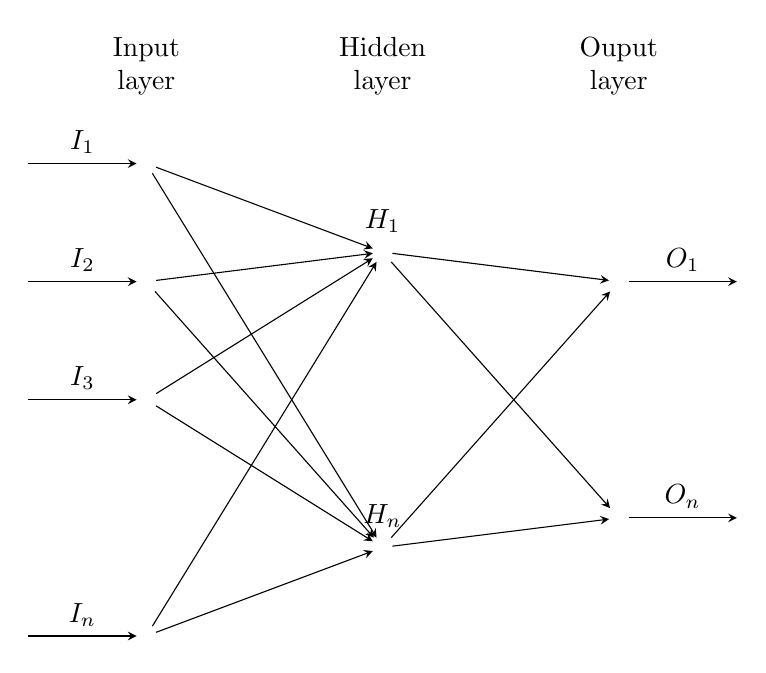
\begin{tikzpicture}[x=1.5cm, y=1.5cm, >=stealth]
				\foreach \m/\l [count=\y] in {1,2,3,missing,4}
				  \node [every neuron/.try, neuron \m/.try] (input-\m) at (0,2.5-\y) {};

				\foreach \m [count=\y] in {1,missing,2}
				  \node [every neuron/.try, neuron \m/.try ] (hidden-\m) at (2,2-\y*1.25) {};

				\foreach \m [count=\y] in {1,missing,2}
				  \node [every neuron/.try, neuron \m/.try ] (output-\m) at (4,1.5-\y) {};

				\foreach \l [count=\i] in {1,2,3,n}
				  \draw [<-] (input-\i) -- ++(-1,0)
				    node [above, midway] {$I_\l$};

				\foreach \l [count=\i] in {1,n}
				  \node [above] at (hidden-\i.north) {$H_\l$};

				\foreach \l [count=\i] in {1,n}
				  \draw [->] (output-\i) -- ++(1,0)
				    node [above, midway] {$O_\l$};

				\foreach \i in {1,...,4}
				  \foreach \j in {1,...,2}
				    \draw [->] (input-\i) -- (hidden-\j);

				\foreach \i in {1,...,2}
				  \foreach \j in {1,...,2}
				    \draw [->] (hidden-\i) -- (output-\j);

				\foreach \l [count=\x from 0] in {Input, Hidden, Ouput}
				  \node [align=center, above] at (\x*2,2) {\l \\ layer};
			\end{tikzpicture}

			\caption{Sketch of a one-hidden-layer artificial neural network model: input $x = \{ x_i | i = 1 \ldots n \}$ and output $y = \{ y_j | j = 1 \ldots m \}$ are connected through a hidden layer $h = \{h_k | j = 1 \ldots p \}$ }
			\label{fig:neuralnet}
		\end{figure}
		Artificial neural networks are a powerful and flexible tool for function approximation. Inspired by biological neurons, there have been numerous questionable claims \wrt their biological plausibility. % cite bishop
		Here, we will treat an artificial network solely as a parametric non-linear function approximator. They can approximate a function $y = f(x)$ with vector input $x = \{ x_i | i = 1 \ldots n \}$ and vector output $y = \{ y_j | j = 1 \ldots m \}$, also see Fig.~\ref{fig:neuralnet}. At minimum they connect the input and the output through one hidden layer $h = \{h_k | j = 1 \ldots p \}$ by:
		\begin{equation} \label{eq1}
			\begin{split}
				h_j & =  a (\sum_i w_{ji} x_i + w_{0i})  \\
				y_j & =  a' (\sum_i w'_{ji} h_i + w'_{0i}),
			\end{split}
		\end{equation}
		with weight matrices $w, w'$, non-linear so-called activation functions $a, a'$  and bias vectors $w_{0}$, $w_{0}'$.
		Neural networks can also comprise multiple hidden layers connect by $h_j  =  a (\sum_i w_{ji} h_i + w_{0i})$.
		It can be shown, that in the limit of infinite hidden units $h_j$ a one-hidden-layer network is enough to approximate any (continuous) function arbitrarily close \cite{cybenko89approx, hornik91approx}.
		In practice, however, networks with more that one layer, referred to as deep neural networks, seem to work better. This may be due to the possibility of building a hierarchical feature representation \cite{zeiler14vis}, that reflects the hierarchical nature of the physical reality.
		Typical activation functions are for example the sigmoid function ($a_{sigm}$ or the rectified linear unit ($a_{relu}$):
		\begin{equation}
			a_{\textrm{sigm}}(x)= \frac{1}{1+e^{-x}}
		\end{equation}
		% \begin{equation}
			% a_{\textrm{tanh}}(x)= \frac{2}{1+e^{-2x} -1 }
		% \end{equation}
		\begin{equation}
			a_{\textrm{relu}}(x)=
			\begin{cases}
			      0 & x\leq 0 \\
			      x & x > 0
			\end{cases}
		\end{equation}
		% \begin{equation}
			% a_{\textrm{elu}}(x)=
			% \begin{cases}
				% e^{-x}-1  & x\leq 0 \\
			      % x & x > 0
			% \end{cases}
		% \end{equation}
		The activation function needs to be non-linear, otherwise the neural network is just a linear classifier (matrix multiplies are again matrices).
		% multiple layers
		 % cite tegmark
		% convolutional
		For processing image data, the weight matrices can be constrained to be only locally connected and to share weights across locations to enforce translation invariance, resulting in \textit{convolutional} neural networks.

		% optimization
		Deep neural networks have highly non-convex likelihood functions, hence for optimization iterative numerical methods are used: The weights $w$ are initialized to some initial value $w^0$ \todo{cite glorot}
		and then updated at time step $t$ with an update rule $w^{t+1}\rightarrow w^t$.
		A simple yet successful rule is given by gradient descent,
		\begin{equation}
			w^{t+1} = w^{t} + \lambda \nabla_{w^t}	 \mathcal{L} (w^t),
		\end{equation}
		where $\lambda$ is the learning rate, parametrizing the step size. In practice, calculating derivatives of the likelihood \wrt the weights can be done efficiently via error backpropagation.
		For big datasets it becomes cumbersome to calculate the gradient w.r.t the whole dataset. Taking only a random subset of the data for an approximation of the gradient, renders the optimization stochastic; the procedure is then called stochastic gradient descent.


\newpage
\section{Generative Models}\label{sec:genmodel}
	\begin{quote}
	    What I cannot create, I do not understand. - R. Feynman
	\end{quote}
	Learning and understanding structure in data by being able to generate, is the rationale behind generative modelling.
	Generative models are mostly applied for unsupervised learning and can be contrasted to discriminative models. While discriminative models are used to model posterior conditionals $p(y|x)$ (\eg for supervised learning (cf. Sec. \ref{sec:supervised}), generative models capture the complete data distribution $p(x)$ in an estimate $\hat p(x)$ \cite{bishop06pattern}. Thus, after estimation, one can generate samples from this model $\hat p$. Hence the name generative model.
	\note{Generative modeling can be used for outlier search, where regions with low probability under the model are taken as indicative for an outlier.}
	The currently predominant generative models are built on either autoencoding or adversarial formulations:

	\subsection{Autoencoding Formulations}\label{sec:autoencoding}
		An autoencoding model is learning by reconstructing samples of data, $\hat x = f(x)$. To enforce data compression (otherwise the identity function is a trivial solution of autoencoding) the function has an information bottleneck, namely an inferred latent code $z$ of reduced dimension. The autoencoder is then the chain of an encoding function $z = e(x)$ and a decoding function $\hat x = d(z) = d(e(x))$.

		Whereas the conventional autoencoder consists of deterministic mappings $e, d$, the {variational autoencoder} \cite{kingma13vae} models the probability distribution $p(x)$. More specifically, it maximizes a lower bound to the logarithmic likelihood $\log p(x)$ of data $x$. This so-called variational lower bound $\mathcal{L}$ is given by:
		% \begin{equation}\label{eq:vae}
			% \mathcal{L} = \underbrace{\mathds{E}_{z\sim q(z|x)}  \log p(x|z)}_{\textrm{reconstruction loss}}  - \underbrace{\textrm{KL}(q(z|x)||p(z))}_{\textrm{regularization}}
		% \end{equation}
		\begin{equation}\label{eq:vae}
			% \mathcal{L} = \mathds{E}_{z\sim q(z|x)}  \log p(x|z) - \textrm{KL}(q(z|x)||p(z))
			\mathcal{L} = \mathds{E}_{z\sim q(z|x)}  \log p(x|z) - \mathds{E}_{z\sim q(z|x)} \log \frac{q(z|x)}{p(z)}
		\end{equation}

		Where $z$ introduces latent variables, with a prior distribution $p(z)$, with an approximation to the posterior $q(z|x)$ of the latent variables, and the posterior of the data given the latent variables $p(x|z)$. If one wants to model the distributions with neural networks, one typically uses Gaussian distributions and lets the networks predict the parameters (mean $\mu$ and variance $\Sigma$) based on the image.
		In the current machine learning contexts, all functions ($e, d$) and moments ($\mu, \Sigma$) are modelled with neural networks.

	\subsection{Adversarial Formulations}\label{sec:adversarial}
		{Generative adversarial networks} (GAN) \cite{goodfellow14gan} consist of two neural networks competing in a zero-sum game. A generator network $G$ is generating images based on a latent code $z$ sampled from a distribution $p(z)$. The discriminator network $D$ is a binary classifier with the task to classify an image as originating from the data distribution $p_{\mathrm{data}}$ or from the distribution produced by $G$. The loss function of $G$ is the negative of the loss of $D$, such that one can formulate the optimization in a minmax form:
		\begin{equation}
			% \begin{split}
			\min_D \max_G - \frac{1}{2} \mathds{E}_{x \sim p_{\mathrm{data}}} [\log D(x)] - \frac{1}{2} \mathds{E}_{z\sim p(z)}[\log (1-D(G(z)))]
			% \end{split}
		\end{equation}
		The generator is then optimized to make the output indiscriminable from the data distribution.
		The discriminator can be interpreted as a learned similarity metric, to measure the closeness of an image to the data distribution \cite{larsen15vaegan}.
		There are many variants and extensions to this basic principle of learning with an adversarial task. For example, one can learn a discriminator for a set of image patches \cite{isola17image2image}. \todo{find more examples, of the gan zoo}

\section{Disentangling Representations}\label{sec:disentangled}
	In supervised learning, a performance measure is naturally induced by the metric, that is being optimized. In the unsupervised setting, judging the performance of a model is less straightforward.
	How to rate the quality of the latent representation?
	\note{For example, when modelling an image domain, one could subjectively rate the quality of the generated image.}
	\todo{introduce latent representation in data compression framing }

	\subsection{Learning Representations}

	\begin{quote}
		{Disentangle as many factors as possible, discarding as little information about the data as is practical.} - Bengio \etal \cite{bengio13rep} % Y. Bengio, A. Courville and P. Vincent \cite{Bengio2013rep}
	\end{quote}

	According to Bengio \etal \cite{bengio13rep}, a representation is useful, if it can be applied to many - in advance unknown - different tasks, while being trained on only one particular task.
	As the downstream tasks can be multifarious, the essential \textit{information} should be contained in the representation.
	For some tasks only a subset of aspects of the data will be necessary, that is why \textit{disentangled factors} make a representation particularly practical.

	The latent representation $z$ learned by generative models captures the essential \textit{information} of the data distribution. That is made sure by requiring the ability to generate samples from the original data distribution from it.
	How then to reach the second goal, the \textit{disentanglement} of generative factors?

	\subsection{Disentangling defined by Equivariance and Invariance}
		\begin{figure}[htp]
			\centering
			% \begin{tikzpicture}
	% % Define nodes
	% \node[obs]                               (x) {$\mathbf{x}$};
	% \node[latent, above=of x, xshift=-1.3cm] (z1) {$\mathbf{z_1}$};
	% \node[latent, above=of x, xshift=1.3cm]   (zn) {$\mathbf{z_N}$};
	% \node[latent, above=of x]   (zi) {$\mathbf{z_i}$};
	% \node[auto=false, above=of x, yshift=0.2cm, xshift=0.7cm] (dots) {$\cdots$}  ;
	% \node[auto=false, above=of x, yshift=0.2cm, xshift=-0.6cm] (dots1) {$\cdots$}  ;
%
	% \node[latent, below=of x, xshift=-1.3cm] (ez1) {$\mathbf{\hat z_1}$};
	% \node[latent, below=of x, xshift=1.3cm]   (ezn) {$\mathbf{\hat z_N}$};
	% \node[latent, below=of x]   (ezi) {$\mathbf{\hat z_i}$};
	% \node[auto=false, below=of x, yshift=0.2cm, xshift=0.7cm] (dots2) {$\cdots$}  ;
	% \node[auto=false, below=of x, yshift=0.2cm, xshift=-0.6cm] (dots3) {$\cdots$}  ;
%
	% \edge {z1,zi,zn} {x} ; %
	% \edge {x} {ez1,ezi,ezn} ; %
	% % Plates
	% % \plate {yx} {(x)(y)} {$N$} ;
	% % \plate {} {(w)(y)(yx.north west)(yx.south west)} {$M$} ;
% \end{tikzpicture}
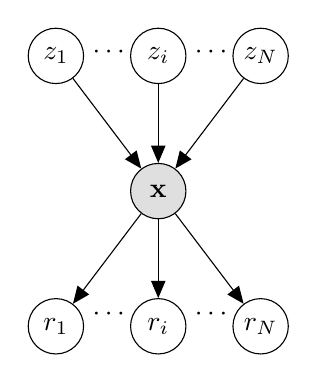
\begin{tikzpicture}
	% Define nodes
	\node[obs]                               (x) {$\mathbf{x}$};
	\node[latent, above=of x, xshift=-1.3cm] (z1) {${z_1}$};
	\node[latent, above=of x, xshift=1.3cm]   (zn) {${z_N}$};
	\node[latent, above=of x]   (zi) {${z_i}$};
	\node[auto=false, above=of x, yshift=0.2cm, xshift=0.7cm] (dots) {$\cdots$}  ;
	\node[auto=false, above=of x, yshift=0.2cm, xshift=-0.6cm] (dots1) {$\cdots$}  ;

	\node[latent, below=of x, xshift=-1.3cm] (ez1) {$r_1$};
	\node[latent, below=of x, xshift=1.3cm]   (ezn) {$r_N$};
	\node[latent, below=of x]   (ezi) {$r_i$};
	\node[auto=false, below=of x, yshift=0.0cm, xshift=0.7cm] (dots2) {$\cdots$}  ;
	\node[auto=false, below=of x, yshift=0.0cm, xshift=-0.6cm] (dots3) {$\cdots$}  ;

	\edge {z1,zi,zn} {x} ; %
	\edge {x} {ez1,ezi,ezn} ; %
	% Plates
	% \plate {yx} {(x)(y)} {$N$} ;
	% \plate {} {(w)(y)(yx.north west)(yx.south west)} {$M$} ;
\end{tikzpicture}


			\caption{Disentangling causal factors means to infer an estimate - \ie a representation - from an image}
			\label{fig:infer}
		\end{figure}

		What is a factor? As outlined in the introduction (cf. Sec. \ref{sec:introduction}), factors in a representation should correspond to causal elements of the world.
		In general, these factors can interact in complicated ways to finally result in an image. Here, we only consider the case where multiple independent factors each have an influence (cf. Fig. \ref{fig:infer}):
		\begin{equation}\label{eq:independent}
			p(z_1 \ldots z_N) = \prod_i p(z_i)
		\end{equation}
		A change in an element, should then lead to: \emph{i)} a corresponding change in the representational factor and \emph{ii)} leave other factors, that represent other elements, unchanged.
		Formally, this can be seen as inference: a number of latent variables ${z_1}\ldots{z_N}$ interacted to cause the existence of the observed image $\mathbf{x}$. The task is now to infer estimates for these latent variables $r(\mathbf{x})_i:=r_i$. A graphical model of the process is shown in Fig.~\ref{fig:infer}.
		A disentangled representation should simultaneously fulfill equivariance and invariance: A change in ${z_i}$ should: \emph{i)} \textit{equivariantly} change in the abstract representational factor $r_i$, \emph{ii)} while leaving the other factors $r_j, j\neq i$, that represent other causes, \textit{invariant}.
		\todo{mathematically,.. $f \circ g (x) = ... $}
		\todo{draw other: arbitrary causal}
		\todo{incorporate definition~\cite{higgins18defdisrep}}


\section{Theoretical Impediments from Causality}\label{sec:causality}


	Generative factors represent causal elements.
	Learning a disentangled representation of generative factors is then understood as causal inference.
	In accordance with the causal literature~\cite{pearl18impediments}, we can make statements about the type of knowledge, that can be gained by the type of data provided. It turns out that from "raw" image data, it is actually impossible to learn a disentangled representation $z$ - raw data referring to images $x$ sampled from $p(x)$, without further assumptions.
	To elucidate this fact, we start with a primer for causal learning (Sec. \ref{sec:causallearning}), outline which inductive biases are needed for disentanglement (Sec. \ref{sec:requirements}) and assess how one can instantiate such biases for disentangling the factors of shape and appearance in images (Sec. \ref{sec:transform}, Sec. \ref{sec:anabysyn})).

	\subsection{Causal Learning}\label{sec:causallearning}
		\begin{figure}[htp]
			\begin{subfigure}{0.3\linewidth}
				\centering
				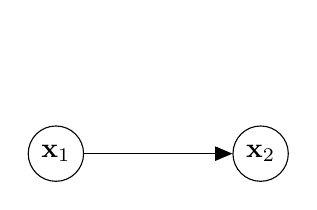
\begin{tikzpicture}
	% Define nodes
	\node[auto=false] (x) {}  ;
	\node[latent, below=of x, xshift=-1.3cm] (s) {$\mathbf{x}_1$};
	\node[latent, below=of x, xshift=1.3cm]   (a) {$\mathbf{x}_2$};
	\edge {s} {a} ; %
	% Plates
	% \plate {yx} {(x)(y)} {$N$} ;
	% \plate {} {(w)(y)(yx.north west)(yx.south west)} {$M$} ;
\end{tikzpicture}



				\caption{}
			\end{subfigure}
			\begin{subfigure}{0.3\linewidth}
				\centering
				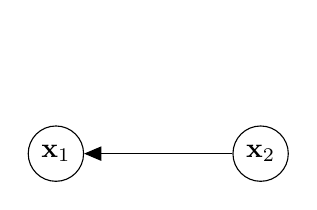
\begin{tikzpicture}
	% Define nodes
	\node[auto=false] (x) {}  ;
	\node[latent, below=of x, xshift=-1.3cm] (s) {$\mathbf{x}_1$};
	\node[latent, below=of x, xshift=1.3cm]   (a) {$\mathbf{x}_2$};
	\edge {a} {s} ; %
	% Plates
	% \plate {yx} {(x)(y)} {$N$} ;
	% \plate {} {(w)(y)(yx.north west)(yx.south west)} {$M$} ;
\end{tikzpicture}



				\caption{}
			\end{subfigure}
			\begin{subfigure}{0.3\linewidth}
				\centering
				\begin{tikzpicture}
	% Define nodes
	\node[obs]                               (z) {$\mathbf{z}$};
	\node[latent, below=of x, xshift=-1.3cm] (x1) {$\mathbf{x}_1$};
	\node[latent, below=of x, xshift=1.3cm]   (x2) {$\mathbf{x}_2$};
	\edge {z} {x1,x2}; %
	% Plates
	% \plate {yx} {(x)(y)} {$N$} ;
	% \plate {} {(w)(y)(yx.north west)(yx.south west)} {$M$} ;
\end{tikzpicture}



				\caption{}
			\end{subfigure}
			\caption{Correlation implies causation - if $x_1$ and $x_2$ correlate, a) $x_1$ may cause $x_2$,  b) $x_1$ may be caused by $x_2$ or c) both are contingent on a latent cause $z$}
			\label{fig:reichenbach}
		\end{figure}

		Learning to infer causality is harder than statistical learning. We outline the basic problem for the case of two variables $x_1, x_2$: statistical learning aims at estimating probabilistic properties such as $p(x_1, x_2)$ or  $p(x_2|x_1)$ from data.
		It is a well-known theme in statistics is that correlation does not imply causation. Less well-known\todo{formulate differently} is Reichenbachs principle \cite{peters17elements, reichenbach56time}, that states: if two random variables are statistically dependent, then there exists a third variable that influences both or a direct causal link between them (Fig. \ref{fig:reichenbach}).
		In addition to estimating the probability distribution, also the causal structure has to be inferred \cite{peters17elements}.

		To show the limitations of raw data, we sketch an intuitive example problem (adapted from \cite{pearl18why}):
		How to learn the causal connection between a barometer and the weather? If the barometer is working well, there exists a clear correlation between the weather condition and the needle position. Given a dataset showing both barometer and corresponding weather condition, a capable machine learning algorithm will be able to capture this correlation. However, it will fail to understand the causal direction, since this is not possible from the data.
		Imagine how a human would go about solving this problem:
		Having a mechanistic model of the world he could reason about the precise causal mechanism relating weather to air pressure to needle position. A simple model could be: weather influences air pressure, pressure influences barometer needle position.
		What if one has no prior knowledge? A solution of child-level simplicity is, to force the needle to move with a finger. Without the power of magic, the weather will not change. Hence causality has to go other way or via a third latent variable influencing both \ie air pressure.
		% There cannot be an abstract intelligence, which finds out about the world purely by observation. The intelligence has to interact with the world, it has to be in the world.
		% e.g.  RCT
		To conclude, the strength of association (correlation) can be estimated with observational data alone, this can answer the question: how likely will it rain, if the barometer needle sinks? But not: how would the weather change if I force the barometer needle to sink?\todo{linking to next section}

		Pearl \cite{pearl18why} distinguishes between three types of questions, that can be answered by different types of knowledge:
		\begin{table}[htp]
			\centering
			\caption{Ladder of causation~\cite{pearl18impediments}. Questions at level $i$ of the ladder are only accessible with information from level $i$ or higher.}
			\label{tab:overview}
			\begin{tabular}{l|ccr}
				\hline
				Level & Symbol & Typical Activity & Typical Questions \\ \hline
				1. Association & $P(y|x)$ & Seeing & What if I see?  \\
				2. Intervention& $P(y|\mathrm{do}(x), z)$ & Doing& What if I do?  \\
				3. Counterfactual& $P(y_x|x', y')$ & Imagining & What if had done?  \\ \hline
			\end{tabular}
		\end{table}

		The levels of this \textit{ladder of causation} \cite{pearl18why, pearl18impediments} are separate not only conceptually, but in the type of data or assumptions that have to be made in order to access them. In particular, by unsupervised learning from observational data only the first level is accessible. The second level requires interactional data or model assumptions, while the third is inaccessible without an explicit model. The answers to these hypothetical questions (counterfactuals) lie by definition not in the data (facts).




	\subsection{Disentangling requires Interventions or Model Assumptions}\label{sec:requirements}
		The results from the study of causal inference also entail that "purely" unsupervised disentangling, \ie estimating $\mathbf{\hat z_i}$ from samples $x \sim p(x)$, is impossible. A proof for this can be found in \cite{locatello18challenging}.
		% so far fitting curve p(x) to data manifold
		Current machine learning operates mostly on the level of association, estimating (complex) correlations from raw data.
		As we have seen, this purely data-driven approach can only go so far.
		In contrast, humans seem to have the ability to interact with their environment and have innate assumptions on coherence, causality, physics etc., which introduce inductive priors~\cite{tenenbaum18think}.
		To bring \emph{i)} interventions and \emph{ii)} model assumptions to our problem of disentangling shape and appearance, we \emph{i)} apply changes to an image, which are assumed to change only one factor and \emph{ii)} model the causal process of the image generation in the theme of analysis-by-synthesis.
		\todo{math}
		% measure: p(x)
		% assume causal model: p(x | a, s)
		% want: p(s | x) and p(a | x)
%
% encoding
% $p(s | x )$
% $p(a | x) = p(a | s, x) p(s | x)$
%
% decoding
% $p(x) = p(x | a, s) p(a) p(s)$
%
% $p(x| do(s), do(a))$



	%&tex
\chapter{Literature Review: Disentangling}

\todo{research for papers connecting disentangling and causality}

\section{Learning Object Shape}
for estimating shape $s$ from images $x$ the task is
$p(s|x)$
representation of shape can be landmarks


Disentangling generative factors definition
model-free vs model-based approaches:
\begin{itemize}
	\item model-based $\rightarrow$ more flexible, transferable, modular combination (like parts)
\end{itemize}
parts as regional attention (cite attention paper)
parts/compositionality is key to creativity -> new combination of known parts

% link to causality: ladder of causal reasoning needs intervention

\section{Analysis-by-Synthesis}
	Capsules, Tieleman
	make model as good as we can implementing as many assumptions as we can and only leave the rest to powerful model
	Synthesis known, analysis only indirectly by observing cognition

	leaving synthesis to learning from scratch, can meet practical/computational limits \eg\ convolutional neural networks better than fully connected neural models.
	But can also be ultimately impossible. Modelling synthesis explicitly with a causal model about image generation, by knowledge about the physical world enables answering interventional and counterfactional questions. (mathematically impossible to learn from ''pure'' data alone)

\section{Causal Learning}
	Pearl
	Ladder of Causation: rung one seen, rung two seeable, rung three cannot be seen.
	Barometer example, best neural network will not know -> theoretical proof (look up in Pearl) -> need interaction with the world / or causal assumptions.

\section{Disentangled Generative Models}
	Capturing essential information about data in a representation by being able to generate it is the rationale behind generative modelling. Currently the approaches in this direction are defined by adversarial \cite{Goodfellow:2014td} and autoencoding \cite{Kingma:2013tz} model formulations. Recently, the endeavour for disentangling explanatory factors in the latent representation is being made explicit in the objective functions \cite{Burgess:2018uf, Chen:2016tp} of these models. So far, however, these attempts are limited to rigid objects without articulation and disentangle holistic image factors like illumination, object rotation or total shape and global appearance. \todo{Denton:2017uf} \ % TODO ref disentangling models % TODO capsules

\section{Disentangling Shape and Appearance}
	Factorizing an object representation into shape and appearance is a popular ansatz for representation learning.
	Recently, a lot of progress has been made in this direction by conditioning generative models on shape information \cite{Esser:2018ue, Ma:2017wq, deBem:2018wp, Ma:2017uu, Siarohin:2018wk, Balakrishnan:2018wo}.
	While most of them explain the object holistically, only few also introduce a factorization into parts \cite{Siarohin:2018wk, Balakrishnan:2018wo}.
	In contrast to these shape-supervised approaches, we learn both shape and appearance without any supervision.

	For unsupervised disentangling, several generative frameworks have been proposed ~\cite{Higgins2016betavae, Chen2016infogan, Li2018analogy, Denton:2017uf, Shu:2018ua, Xing:2018un}.
	However, these works use holistic models and show results on rather rigid objects and simple datasets, while we explicitly tackle strong articulation with a part-based formulation.

\section{Part-based Representation Learning}
	Describing an object as an assembly of parts is a classical paradigm for learning an object representation in computer vision \cite{Ross:2006uc} with linkage to human perceptual theories \cite{Biederman:1987tc}.
	What constitutes a part, is the defining question in this scheme.
	Defining parts by e.g. (\emph{i}) visual/semantic features (object detection), or by (\emph{ii}) geometric shape, behavior under (\emph{iii}) viewpoint changes or (\emph{iv}) object articulation, in general leads to a different partition of the object.
	Recently, most part learning has been employed for object recognition, such as in \cite{Felzenszwalb:2010ve, Novotny:2017ta, Singh:2012un, Mesnil:2013hi, Yang:2016uo, Lam:2017ta}.
	% other methods for discriminative -> recognition -> focus on visual factorization % ours for generative image modeling -> also structural aspects %\cite{DPM, constellation1,constellation2} combine parts with a probabilistic prior on their spatial arrangements. %Novotny et al. \cite{anchornet} find parts shared by similar categories to perform semantic matching. Mining of discriminative parts can be formulated as an clustering problem or an iterative refinement process \cite{partLearning2}.
	To solve such a discriminative task, parts will be based on the semantic connection to the object and can ignore their spatial arrangement and articulation of the object instance. Our method instead is driven by a generative process and aims at more generic modeling of the object as a whole. Hence, parts have to encode both spatial structure and visual appearance accurately. To our best knowledge unsupervised part learning and the proposed split in shape and appearance description for a part has only been used in pre-deep learning approaches \cite{Ross:2006uc, Nguyen:2013vk, Cootes:1998tn}.


\section{Landmark Learning}
	There is an extensive literature on landmarks as compact representations of object structure.
	Most approaches, however, make use of manual landmark annotations as supervision signal \cite{Wu:2017vc, Ranjan:2016vv, Yu:2016vi, Zhang:2016vx, Zhu:2015tz, Zhang:2014wy, Pedersoli:2014ta, Ionescu:2011ue, Toshev:2014tp, Pfister:2015uo, Wei:2016ws, Newell:2016vq, Lim:2018uo, Cao:2017vv}.

	To tackle the problem without supervision, Thewlis \etal \cite{Thewlis:2017wi} proposed enforcing equivariance of landmark locations under artificial transformations of images. The equivariance idea had been formulated in earlier work \cite{Lenc:2016tz} and has since been extended to learn a dense object-centric coordinate frame \cite{Thewlis:2017wg}. However, enforcing only equivariance encourages consistent landmarks at %easily
	discriminable object locations,
	but disregards an explanatory coverage of the object.
	% which is especially critical for strong
	%does not aim at explaining the object from it.

	Zhang \etal \cite{Zhang:2018vz} addresses this issue: the equivariance task is supplemented by a reconstruction task in an autoencoder framework, which gives visual meaning to the landmarks. However, in contrast to our work, he does not disentangle shape and appearance of the object. Furthermore, his approach relies on a separation constraint in order to avoid the collapse of landmarks.
	This constraint results in an artificial, rather grid-like layout of landmarks, that does not scale to complex articulations.
	%In contrast, our method disentangles shape and appearance. Hence, for optimal reconstruction, our model has to make use of the shape information efficiently, which leads to a meaningful coverage.

	%Building on the reconstruction objective introduced by \cite{Zhang:2018vz},
	Jakab \etal \cite{Jakab:2018wc} proposes conditioning the generation on a landmark representation from another image. A global feature representation of one image is combined with the landmark positions of another image to reconstruct the latter. Instead of considering landmarks which only form a representation for spatial object structure, we factorize an object into local parts, each with its own shape \textit{and} appearance description.
	Thus, parts are learned which meaningfully capture the variance of an object class in shape as well as in appearance.

	Additionally, and in contrast to all these works (\cite{Thewlis:2017wi, Zhang:2018vz, Jakab:2018wc}) we take the extend of parts into account, when formulating our equivariance constraint. Furthermore, we explicitly address the goal of disentangling shape and appearance on a part-based level by introducing invariance constraints.
	%
	%
	%Jakab \etal \cite{Jakab:2018wc} proposes conditioning the generation on a landmark representation from another image. A global feature representation of one image is combined with the landmark positions of another image to reconstruct the latter.
	%In contrast to our work, appearance representation is global, whereas we partition an object explicitly into local parts, each with its own shape \textit{and} appearance description. The conceptual difference here is, that we understand a part not only as a point (landmark), but as an image region, with an appearance description for this region. This %further factorization
	%encourages part placement at visually meaningful locations and assists the part assignment consistency.
	%\\
    %In contrast to all these works (\cite{Thewlis:2017wi, Zhang:2018vz, Jakab:2018wc}) we model shape by parts with an extend. That extend needs to be equivariant up to the second moment and is used to extract the appearance of a part, which leads to better object coverage. In addition, we make the goal of disentangling explicit with our formulation and show quantitative results on this.
    %\textbf{Landmark learning.}
	%There is an extensive literature on landmarks as compact representations of object structure.
	%Most approaches, however, make use of manual landmark annotations as supervision signal \cite{Wu:2017vc, Ranjan:2016vv, Yu:2016vi, Zhang:2016vx, Zhu:2015tz, Zhang:2014wy, Pedersoli:2014ta, Ionescu:2011ue, Toshev:2014tp, Pfister:2015uo, Wei:2016ws, Newell:2016vq, Lim:2018uo, Cao:2017vv}.
	%\\
	%To tackle the problem without supervision, Thewlis \etal \cite{Thewlis:2017wi} proposed enforcing equivariance of landmark locations under artificial transformations of images. The equivariance idea had been formulated in earlier work \cite{Lenc:2016tz} and has since been extended to learn a dense object-centric coordinate frame \cite{Thewlis:2017wg}. However, enforcing only equivariance encourages consistent landmarks at easily discriminable object locations, but disregards a sensible coverage of the object.
	%\\
	%Zhang \etal \cite{Zhang:2018vz} addresses this issue: the equivariance task is supplemented by a reconstruction task in an auto-encoder framework, which gives visual meaning to the landmarks. However, their approach does not disentangle shape from appearance, thus shape information can be encoded in the appearance representation resulting in the collapse of the landmarks. To counter this they rely on a artificial separation constraint which results in an artificial, rather grid-like layout of landmarks, that does not scale to complex variation in object shape.
	%In contrast, our method disentangles shape and appearance of the object and thus, for optimal reconstruction, our model has to capture the variation of object shape in the shape representation which automatically leads to a meaningful object coverage.
	%\\
    %Jakab \etal \cite{Jakab:2018wc} proposes conditioning the generation on a landmark representation from another image. A global feature representation of one image is combined with the landmark positions of another image to reconstruct the latter. Instead of considering landmarks which only form a representation for spatial object structure, we factorize an object into local parts, each with its own shape \textit{and} appearance description.
	% Thus, parts are learned which meaningfully capture the variance in shape as well as in appearance of an object class.
    %In contrast to all these works (\cite{Thewlis:2017wi, Zhang:2018vz, Jakab:2018wc}) we take the extend of parts into account when formulation the equivariance constraint.
    % In addition, we make the goal of disentangling shape and appearance on a part based level explicit with our formulation and show quantitative results on this.

	\chapter{Method}
% describe method

% INTRO FIGURE: PART REPRESENTATION
% \begin{figure}[t]
	% \begin{subfigure}{0.3\linewidth}
	% \centering
	% \includegraphics[trim={0cm 0cm 0cm 0cm},clip, width=1.\linewidth]{fig/rep1_hq}\caption{}
	% \end{subfigure}
	% \begin{subfigure}{0.3\linewidth}
	% \centering
	% \includegraphics[trim={0cm 0cm 0cm 0cm},clip, width=1.\linewidth]{fig/rep2}\caption{}
	% \end{subfigure}
	% \begin{subfigure}{0.3\linewidth}
	% \centering
	% \includegraphics[trim={0cm 0cm 0cm 0cm},clip, width=1.\linewidth]{fig/rep3}\caption{}
	% \end{subfigure}
	% \caption{An object is represented in parts. Each part has a distinct spatial extend (part shape) and a corresponding feature descriptor (part appearance). (a) input image, (b) model output of part shapes (each plotted in a different color), (c) schematic illustration of part appearances}
	% \label{fig:representation}
% \end{figure}
	\todo{representation figure}
	\todo{link to disentangling, causality stronger}
	To capture an object in an abstract representation, we follow two key ideas: \emph{(i)} disassembling the object into its constituent parts and \emph{(ii)} disentangling spatial geometry (shape) from visual features (appearance). Hence, we model an object as a composition of parts, each part with a part appearance and a part shape, as sketched in Fig. \ref{fig:representation}. The part shape should correspond to the area in the image where the part is located, whereas the part appearance is a feature descriptor for that area. The overall object representation is then the collection of part shapes and part appearances. \\
	% \begin{equation}
	%(a, s) = \cu{\sigma}_i ({\alpha}_i, {\sigma}_i)
	%\end{equation}
	%\label{eq:representation}
	% enforcing locality of parts is important
	% what do our representations entangle still?:
	% shape: position, shape, size
	% appearance: illumination, color, texture, material
	The disentanglement of shape and appearance can be enforced by demanding that shape is invariant under the transformation of appearance and vice versa. This is realized in a two-stream autoencoding formulation. Here, an image is reconstructed from a combination of shape and appearance, with shape extracted from the appearance-transformed image and appearance from a shape-transformed image. Additionally, the part shape is tied to the location of the part in the image: an equivariance loss encourages that the part shape moves in unison with the part in the image. We implement these objectives into a loss framework, which is explained in sec. \ref{sec:framework}. \\
	To assert a decomposition into independent local parts, we ensure their local modelling and treatment throughout the whole pipeline. This is highlighted when describing the architecture in sec. \ref{sec:architecture}.

	\begin{figure}[htp]
		\centering
		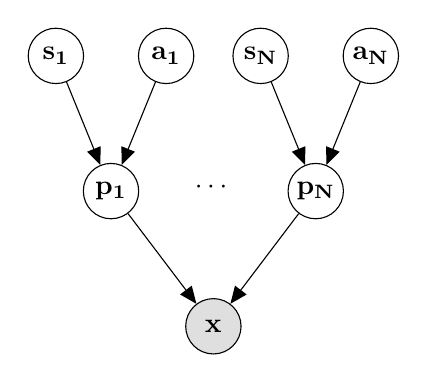
\begin{tikzpicture}
	% Define nodes
	\node[obs]                               (x) {$\mathbf{x}$};
	\node[latent, above=of x, xshift=-1.3cm] (z1) {$\mathbf{p_1}$};
	\node[latent, above=of x, xshift=1.3cm]   (zn) {$\mathbf{p_N}$};
	\node[latent, above=of zn, xshift=-0.7cm]   (sn) {$\mathbf{s_N}$};
	\node[latent, above=of zn, xshift=0.7cm]   (an) {$\mathbf{a_N}$};
	\node[latent, above=of z1, xshift=-0.7cm]   (s1) {$\mathbf{s_1}$};
	\node[latent, above=of z1, xshift=0.7cm]   (a1) {$\mathbf{a_1}$};
	% \node[latent, above=of x]   (zi) {$\mathbf{p_i}$};
	\node[auto=false, above=of x, yshift=0.2cm] (dots) {$\cdots$}  ;
	% \node[auto=false, above=of x, yshift=0.2cm, xshift=-0.6cm] (dots1) {$\cdots$}  ;
	% Connect the nodes
	\edge {z1,zn} {x} ; %
	\edge {a1,s1} {z1} ; %
	\edge {an,sn} {zn} ; %
	% Plates
	% \plate {yx} {(x)(y)} {$N$} ;
	% \plate {} {(w)(y)(yx.north west)(yx.south west)} {$M$} ;
\end{tikzpicture}


		\caption{Modelling an image $\mathbf{x}$ of an object with shape ${\sigma}_{\mathbf{x}}$ and appearance $\alpha_{\mathbf{x}}$, by factorizing into part shapes ${{\sigma}}^i_{\mathbf{x}}$ and part appearances ${\alpha}^i_{\mathbf{x}}$}
		\label{fig:representation}
	\end{figure}

\section{Transformation Framework}\label{sec:framework}
	% CROSSING TASK FRAMEWORK
	\begin{figure}[t]
		\centering
		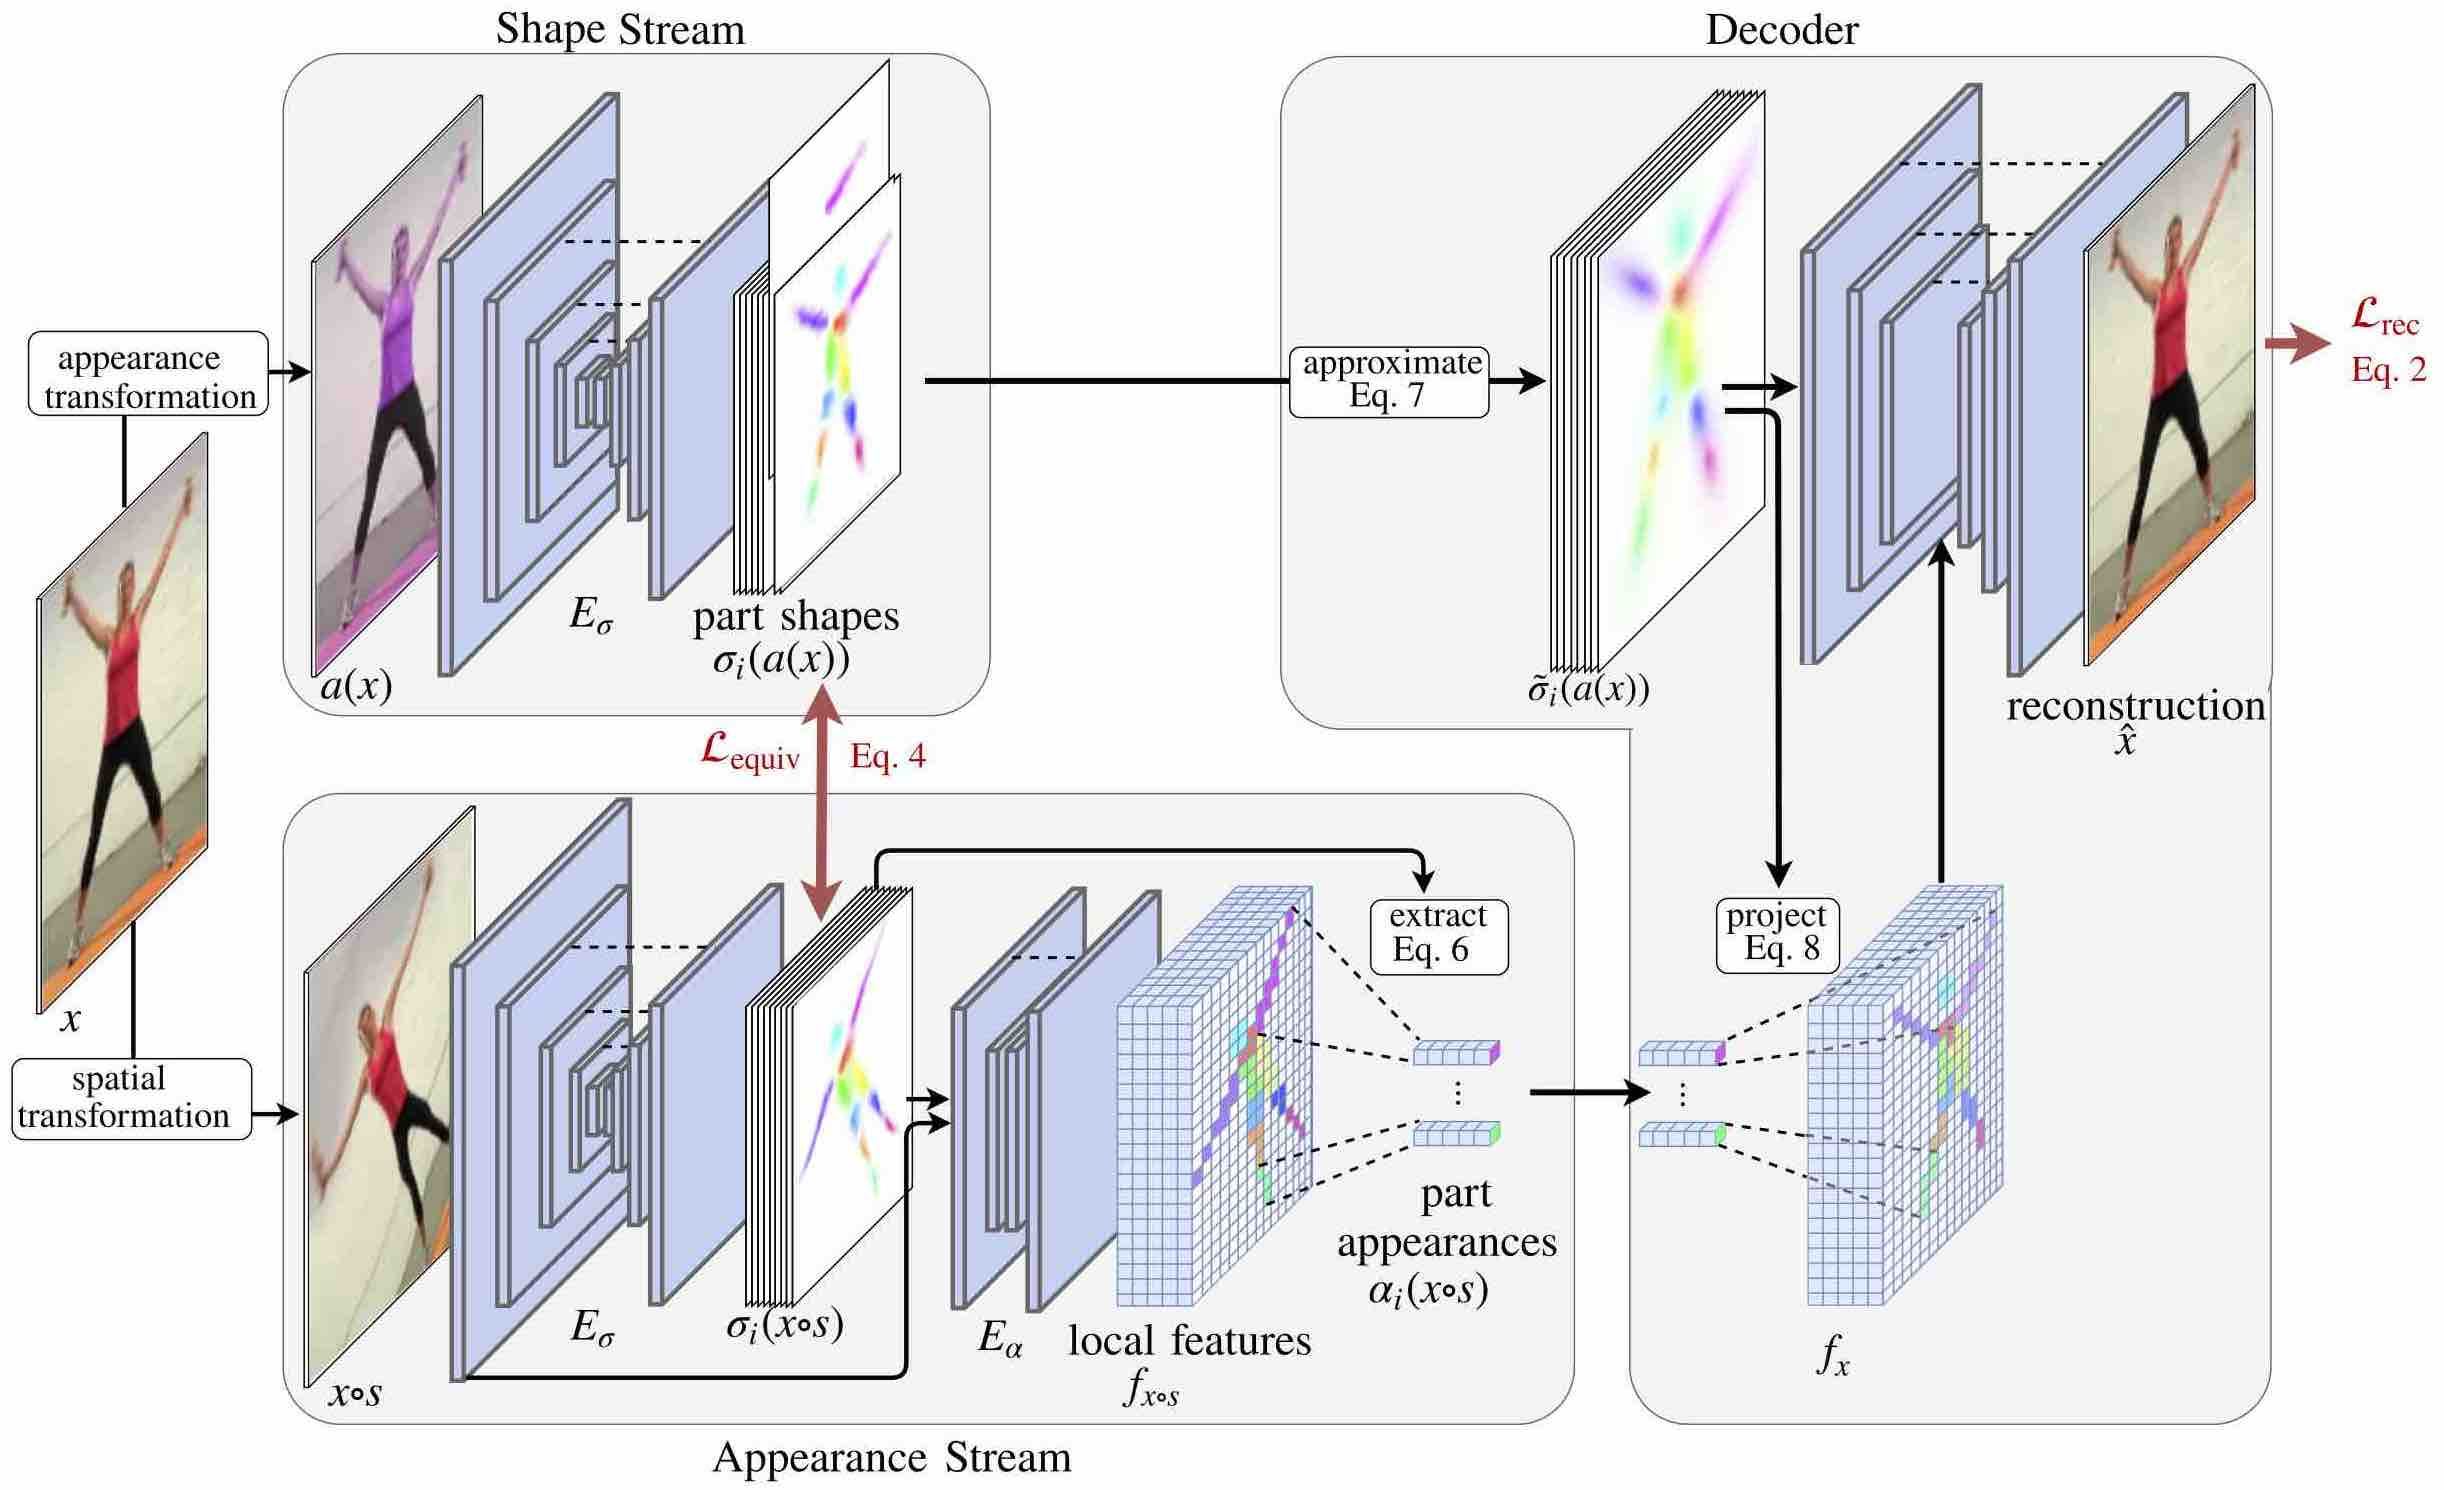
\includegraphics[trim={0cm 0cm 0cm 0cm},clip, width=1.\linewidth]{fig/other/architecture_final}
		\caption{Encoder $E$ encodes shape and appearance for two transformed images $s(\mathbf{x})$ and $a(\mathbf{x})$, after recombination $R$ of $({\alpha}_{s(\mathbf{x})}, {\sigma}_{a(\mathbf{x})})$ into latent image $Z$, the decoder $D$ reconstructs the image $\mathbf{x}$.}
		\label{fig:architecture}
	\end{figure}
	%Definitions
	We want to represent an object in an image $\mathbf{x}$. Let us denote the part shape for part $i$ with ${\sigma}^i_\mathbf{x}$ and the part appearance with ${\alpha}^i_\mathbf{x}$. For an object with $n$ parts, the overall shape is constituted by the collection of its part shapes ${\sigma}_\mathbf{x} =  ({\sigma}^1_\mathbf{x}, ...,  {\sigma}^n_\mathbf{x})$, the same goes for the appearance ${\alpha}_\mathbf{x} =  (\alpha^1_\mathbf{x}, ...,  \alpha^n_\mathbf{x})$. We model the part appearances as feature vectors, the part shapes are chosen to be scalar fields like the image itself. Thereby one can establish a direct correspondence of locations in the image to locations in the shape representation.\todo{say the following or not?}\\
	%In contrast to other works, where object pose is often modeled by single points as landmarks, a representation based on a scalar field is much richer: whereas a landmarks inform about the exact position, the field-like representation also describes the size and shape of the object parts (see Fig.\ref{fig:representation}).
	% Transformations -> Crossing framework
	How do we disentangle the shape and appearance components in the representation? In general, a variation in shape will not affect appearance and vice versa. Thus, if we deliberately change shape without changing appearance, we can enforce the invariance of the appearance representation under such a change.
	We refer to these changes as shape transformations $s: \mathbf{x} \rightarrow s(\mathbf{x})$, which, if applied to an image $\mathbf{x}$, directly act on the underlying pixel space $\Lambda$.
	Along the same lines we can define appearance transformations $a: \mathbf{x} \rightarrow a(\mathbf{x})$, which act on the image itself.
	The shape should be invariant under change of appearance, conversely, the appearance should be invariant under change of shape.
	In addition, the shape should transform in the same manner as the image.
	That means the shape representation is assumed to be equivariant under shape transformations.
	In summary:
	\begin{align}
		{\alpha}_{s(\mathbf{x})}  &= {\alpha}_{\mathbf{x}} \tag{invariance of appearance}\\
		{\sigma}_{a(\mathbf{x})} &= {\sigma}_{\mathbf{x}}  \tag{invariance of shape}\\
		{\sigma}_{s(\mathbf{x})} &= s({\sigma}_{\mathbf{x}}) \tag{equivariance of shape}
	\label{eq:invar}
	\end{align} % quad \forall i \leq n
	Our method builds on the autoencoding paradigm, with part shapes and part appearances assuming the role of the latent code.
	To incorporate these constraints into the loss of an autoencoder, we reconstruct an image $\mathbf{x}$ not from the shape and appearance $({\alpha}_\mathbf{x}, {\sigma}_\mathbf{x})$ determined from the original image $\mathbf{x}$, but from appropriately transformed images $({\alpha}_{s(\mathbf{x})}, {\sigma}_{a(\mathbf{x})})$.
	If the invariance constraints, as formulated above, are full-filled, these transformations do not change the latent code.
	Thus, the loss implicitly enforces invariance.
	To obtain shape and appearance, we encode both $a(\mathbf{x})$ and $s(\mathbf{x})$ with an encoder $\mathrm{E}$.
	And, after a recombination (for details see sec. \ref{sec:architecture}) to a latent image $Z$, a decoder $\mathrm{D}$ reconstructs the image.
	This configuration is depicted in Fig. \ref{fig:architecture}, the reconstruction loss $\mathcal{L}_{\textrm{rec}}$ is as follows:
	%\begin{align}
	%\mathcal{L}_{\textrm{rec}} &=  \lVert X -  \mathrm{D}[\mathrm{R}[\mathrm{E}(\mathbf{x})]]\rVert \\
	%&= \lVert  X  - \mathrm{D}[\mathrm{R}[ ({\alpha}_{\mathbf{x}}, {\sigma}_{\mathbf{x}})]]\rVert \nonumber \\
	%&= \lVert  X  - \mathrm{D}[\mathrm{R}[ ({\alpha}_{X_{\pi'}}, {\sigma}_{X_{\phi'}}]]\rVert \nonumber
	%\end{align}
	%The to-be-reconstructed image $X_{\phi, \pi}$ has been subject to shape and appearance transformations $X \rightarrow \phi \circ \pi (\mathbf{x})$.
	%We instantiate this loss in a two-stream configuration, as shown in Fig. \ref{fig:framework}. %Encoder and decoder are the same for each stream, but image representations are crossed.
	%For simplicity we abbreviate \alpha = {\alpha}_{s(\mathbf{x})}$, \alpha' = {\alpha}_{a(\mathbf{x})}$ , $s = {\sigma}_{a(\mathbf{x})}$ and $s' = {\sigma}_{\pi (\mathbf{x})}$.
	%In accordance with the desired invariances, one can apply a transformation $\phi$ to the image, in order to selectively destroy appearance information in the shape representation and vice versa destroy shape information in the appearance representation with $\pi$.
	%The first stream encodes $s(\mathbf{x})$ to obtain $(a, s')$  and the second stream encodes $a(\mathbf{x})$ to obtain $(a', s)$.
	%Then appearance and shape representations are crossed.
	%After recombining $(a, s)$ to a feature volume $V$ (explained in detail in sec. \ref{sec:architecture}), the decoder reconstructs $\mathbf{x}$.
	\begin{equation}
	\mathcal{L}_{\textrm{rec}}= \lVert  \mathbf{x}  - \mathrm{D}[{\alpha}_{s(\mathbf{x})}, {\sigma}_{a(\mathbf{x})}]\rVert
	\end{equation}
	\label{eq:loss_rec}
	%From an information perspective, we apply an appearance transformation to the image, to selectively destroy appearance information in the shape representation and vice versa destroy shape information in the appearance representation with a shape transformation.
	Let us examine what this formulation means on the level of a single part: the part appearance $\alpha^i_{\mathbf{x}}$ is extracted at locations in the spatially transformed image ${\sigma}^i_{s(\mathbf{x})}$, but then used for reconstruction at the location in the original image ${\sigma}^i_{\mathbf{x}}$. For example in Fig.  \ref{fig:architecture} the appearance of the arm will be extracted in a raised position, but then these features are used for reconstructing an arm in a lowered position. For this to succeed, firstly, the appearance features need to be sufficiently abstract. Secondly, part locations of the two images have to refer to the same part and track the location of it consistently. This part assignment consistency is an implicit way to improve equivariance under the shape transformations.\\
	%The shape also need to be invariant under appearance transformations, so part assignment needs to be consistent .
	%For video data the crossing task can be run on images pairs that show the same object in a different articulation (i.e. different frames of the video), enforcing equivariance of $s$ with respect to natural shape transformations. \\
	For a known shape transformation the equivariance of shape can also be encouraged explicitly with a loss. This has been used before in the context of unsupervised landmark learning by \cite{thewlis17, zhang18} as a point-wise loss on a part probability map, encouraging the exact location of a part to transform accordingly. In our case, the part shapes shall not encode probability, but instead the spatial extend of a part. In approximation, we want the first two moments ($\mu, \Sigma$) to transform correctly. Thereby the extend and orientation of the parts is penalized in addition to its mere position.
	\begin{equation}
	\mathcal{L}_{\textrm{equiv}}^i = \mathcal{L}_{\mu}^i+ \mathcal{L}_{\Sigma}^i
	\label{covariance}
	\end{equation}
	The overall loss objective is the sum of the reconstruction loss and the equivariance loss for all $n$ parts:
	\begin{equation}
	\mathcal{L} = \sum_{i=1}^n \mathcal{L}_{\text{equiv}}^i + \mathcal{L}_{\textrm{rec}}
	\end{equation}


\section{Analysis-by-Synthesis Architecture}\label{sec:architecture}
	The autoencoding pipeline consists of analysis into factors and subsequent synthesis. The \textbf{analysis} is the {encoding} of both shape and appearance for each part. The \textbf{synthesis} is the meaningful {recombination} of this information into a latent image and the {decoding} of this latent image to reconstruct the image. %The whole process is sketched in Fig. \ref{fig:framework}, the operations in more detail are visualized in Fig. \ref{fig:architecture}.
	Throughout the procedure we maintain the local correspondence between the representation and the image: We ensure a local appearance extraction in the encoding, a local synthesis in the recombining and a local usage of the latent image in the decoding. These architectural restrictions enable a disentangled part representation with the interpretation of a part as a localized entity. \\

	\subsection{Analysis}

		The encoding of shape and appearance given an image ${(\alpha, \sigma | \mathbf{x})}$\footnote{ For a slim notation, we leave out the explicit reference to the generic input image $\mathbf{x}$ in this section: $\alpha, \sigma, \alpha^i, {\sigma}^i$ refer to ${\alpha}_\mathbf{x}, {\sigma}_{\mathbf{x}}, \alpha^i_{\mathbf{x}}, {\sigma}i_{\mathbf{x}}$.} proceeds in two steps: \\
		\emph{(i)} $(\sigma |\mathbf{x})$: The part shapes are predicted given the image. To extract part shapes we use an hourglass neural network. We utilize the hourglass in both steps, as this model is able to preserve pixel-wise locality, and also integrates information from multiple scales \cite{newell16hourglass}. The network input is an image $\mathbf{x}$, the output a stack of $n$ part shapes $\sigma =  \{ {\sigma}^i| i=1, ...,  n\}$.\\
		\emph{(ii)} $(\sigma| \alpha , \mathbf{x})$: The part appearances $\alpha =  \{\alpha^i \vert i=1, ...,  n\}$ are predicted given the image and the part shapes. Again we use an hourglass network, albeit shallower. The input is the original image concatenated with the stack of part shapes. The output is a feature stack $F$. A part appearance is obtained by averaging the feature stack with the a part shape:
		\begin{equation}
			\alpha^i = \sum_{p \in \Lambda} A(p) \frac{{\sigma}^i(p)}{\sum_{p' \in \Lambda}{\sigma}^i(p')}.
		\end{equation}
		Each $\alpha^i$ now describes the appearance of a part spatially localized by the part shape ${\sigma}^i$. \\


	\subsection{Synthesis}
		In the analysis-by-synthesis regime, once the object representation is successfully factorized, one can make assumptions on how the factors reunite to generate an image, following the knowledge and intuition about how objects give rise to images in the physical world (cf.\ sec. \ref{sec:anabysyn}).


		Firstly, we re-merge shape and appearance into images of descriptors at the correct locations. For each part, appearance is multiplied with the corresponding shape, yielding $n$ part feature images:
		\begin{equation}
			z^i(\mathbf{x}) = {\sigma}^i(\mathbf{x}) \cdot \alpha^i .
		\end{equation}


		Secondly, we reassemble the object from its parts: the part feature images $z^i$ are summarized by summing in a single image:
		\begin{equation}
			Z(x) = \sum_i \frac{z^i(\mathbf{x})}{1 + \sum_j z^j(\mathbf{x})}.
		\end{equation}
		The result is an image of part feature descriptors located according to their corresponding part shape, which we call latent image $Z$.
		\note{What is the rationale behind this approach?}
		Finally, the latent image needs to be decoded to an image. This is done by a neural network decoder. The decoder architecture is modeled after the up-sampling stream of a standard U-Net \cite{ronneberger15unet}. The latent image is scaled to different resolutions\todo{alter figure z1 etc} and inserted, after each layer, in addition to the part shapes\todo{ why add shapes?}. As before, the crucial property of the parts that needs to be conserved is their local direct correspondence to the image. On the one hand, one needs to assure, that the receptive field of the neurons does not extend to the full image, in order to thwart a complex non-local interaction of part information. This is why we use only half of a U-Net instead of a complete U-Net or an hourglass architecture.
		On the other hand, it is essential to regularize the information already before passing it to the decoder. Keeping in mind that the part shape should be of rather simple geometry, we introduce a differentiable information bottlenecks, in order to prevent the shape from being scattered over the object. It is an approximation of the part shape as
		\begin{equation}\label{eq:approx}
			\hat {\sigma}^i(x) = \frac{1}{1 + (\mathbf{x} -\mu)^T \Sigma^{-1} (\mathbf{x} - \mu)},
		\end{equation}
		where $\mu$ and $\Sigma$ are the mean and the covariance matrix of the part shape ${\sigma}^i$. This allows to pass second-order information such as size and orientation of the part to the decoder. Note that all operations are fully differentiable, such that a gradient-based optimization is possible.


	\section{Implementation Details}\label{sec:implementationdetails}
		The image resolution is $128 \times 128$, but the resolution of corresponding part shapes is $ 64 \times 64$.
		For the reconstruction  loss $\mathcal{L}_\text{rec}$ we use the $L_1$ or $L_2$ distance.
		To prevent parts from trying to explain the whole image, instead of focusing on the object, we also restrict the reconstruction loss to an area around the part shape: a sum of Gaussian approximations around the means of the part shapes is folded with the loss.\\
		In the decoder, the latent image Z is not only rescaled, but also filled with parts incrementally.
		At the lowest scale only some parts are inserted, with each scale parts are added until at the highest scale all parts are used. This makes the part decoding a hierarchical process. The underlying assumption is, that parts exist at multiple scales.
		For landmark learning, we approximate the part shapes in the decoder in the bottleneck also with eq. \ref{eq:approx}, but fix the covariance $\Sigma$ to be the identity matrix.
		Hence, effectively only information about the mean of each part shape can reach the decoder. This mean information is used as a landmark, so encouraging an accurate estimation of the mean through reconstruction is wanted.\todo{this needs further explanation or is dangerous}\\
		To instantiate shape transformations $s$, one needs image pairs that show the same object in a different articulation or position: For static images an artificial thin-plate spline transform (TPS) can be applied, which generalizes rotation, scaling, translation.
		For video data adjacent frames exhibit natural shape transformations.
		The appearance transformation $a$ is encompassing a color augmentation, contrast variations, and changes in brightness.
		In general, the more selective the transformation distinguishes shape and appearance, the more invariant the representation\note{ more on this in experimental section}.

	%&tex
\chapter{Experiments}
%
\begin{table}
	\centering
	\caption{Difficulties of datasets: articulation, intra-class variance, background clutter and viewpoint variation}
	\label{tab:challenges}
	\begin{tabular}{l|rrrr}
		Dataset &  Articul.& Var. &  Backgr.& Viewp.  \\ \hline
		CelebA &   &  &  &    \\
		Cat Head & &  \checkmark&  &   \\
		CUB-200-2011 & & \checkmark& \checkmark&   \\
		Human3.6M &\checkmark& &  & \checkmark  \\
		BBC Pose &  \checkmark&  & \checkmark&  \\
		Dogs Run & \checkmark& \checkmark& \checkmark&   \\
		Penn Action & \checkmark& \checkmark& \checkmark& \checkmark\\
	\end{tabular}
\end{table}
%
% SHOW DISENTANGLING: SHAPE
\begin{figure}[t]
	\begin{subfigure}{0.5\textwidth}
	\centering
	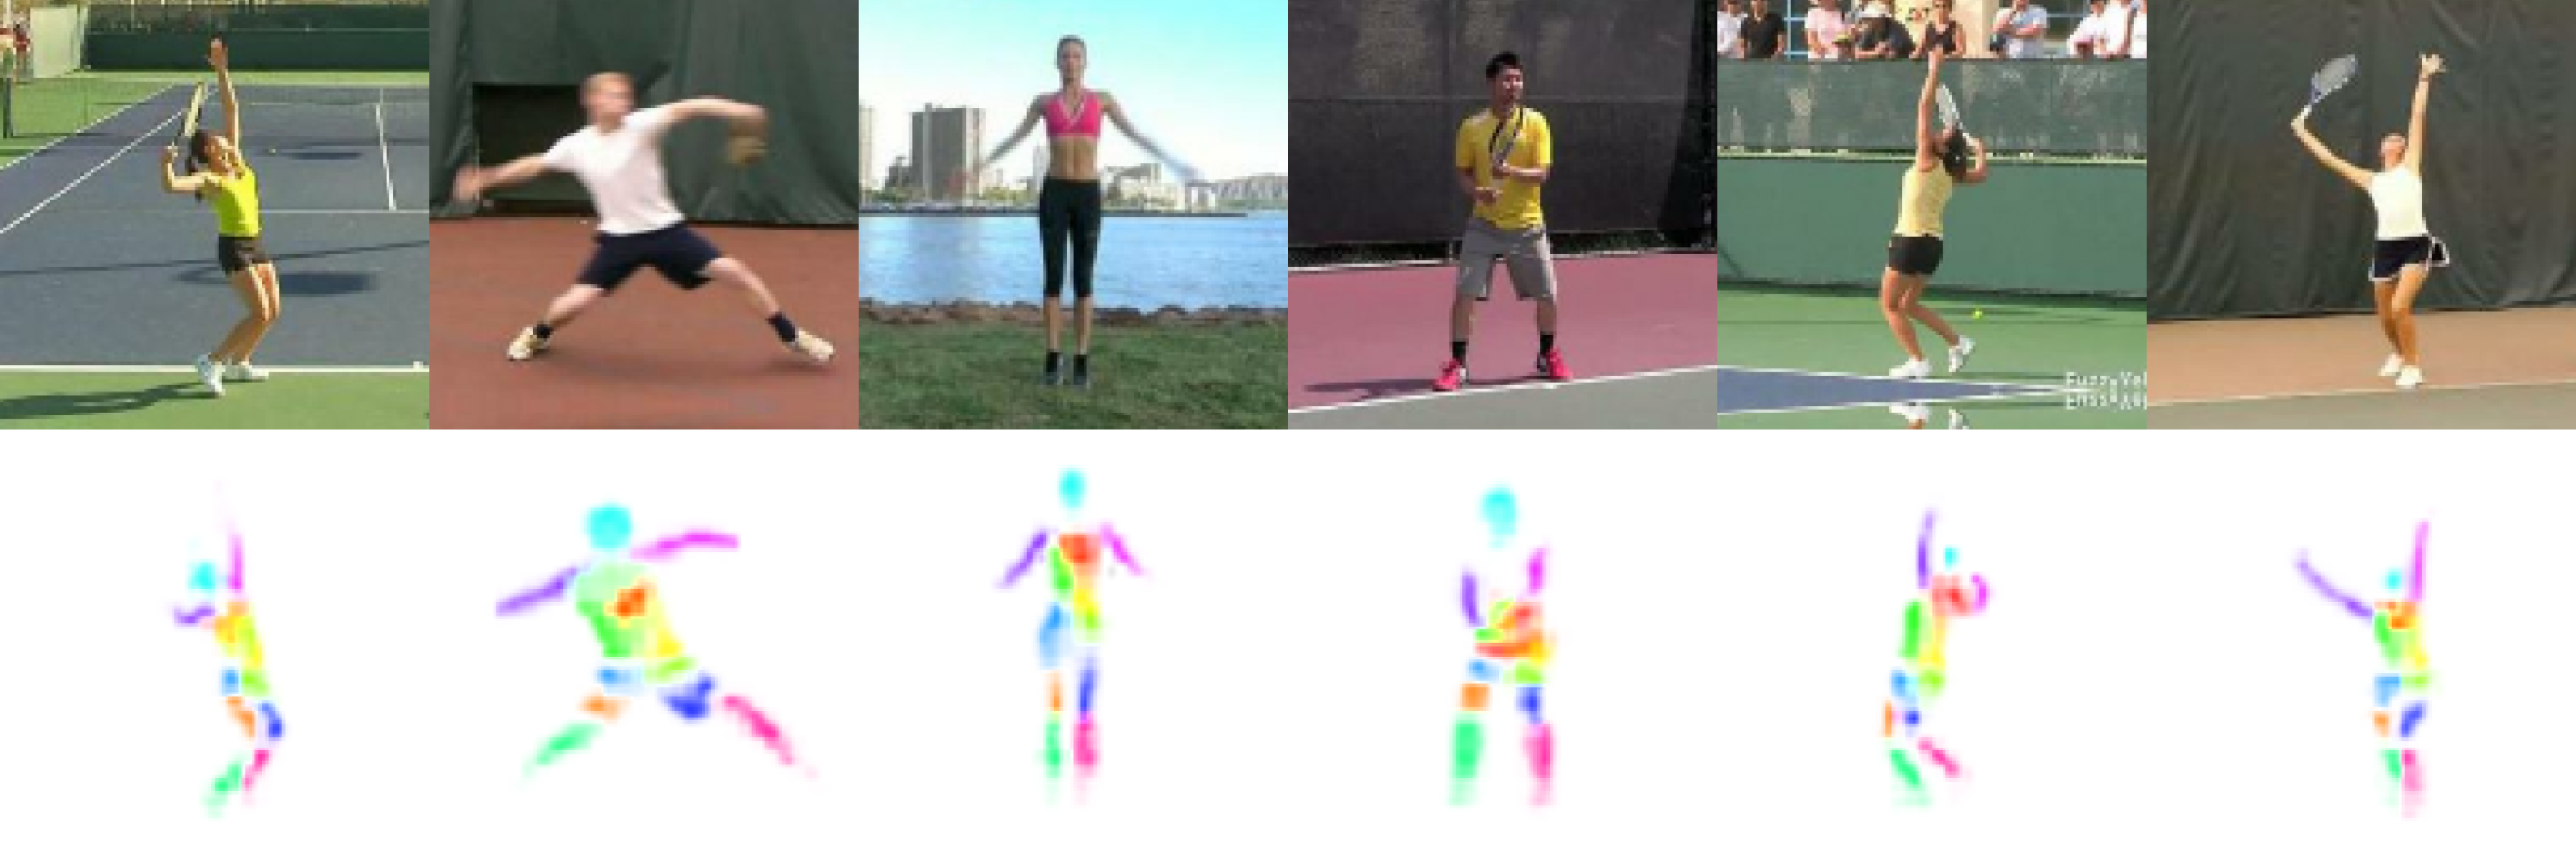
\includegraphics[trim={0cm 0cm 0cm 0cm},clip, width=1.\linewidth]{fig/shape6white}\caption{}
	\label{fig:shape_penn}
	\end{subfigure}
	\begin{subfigure}{0.5\textwidth}
	\centering
	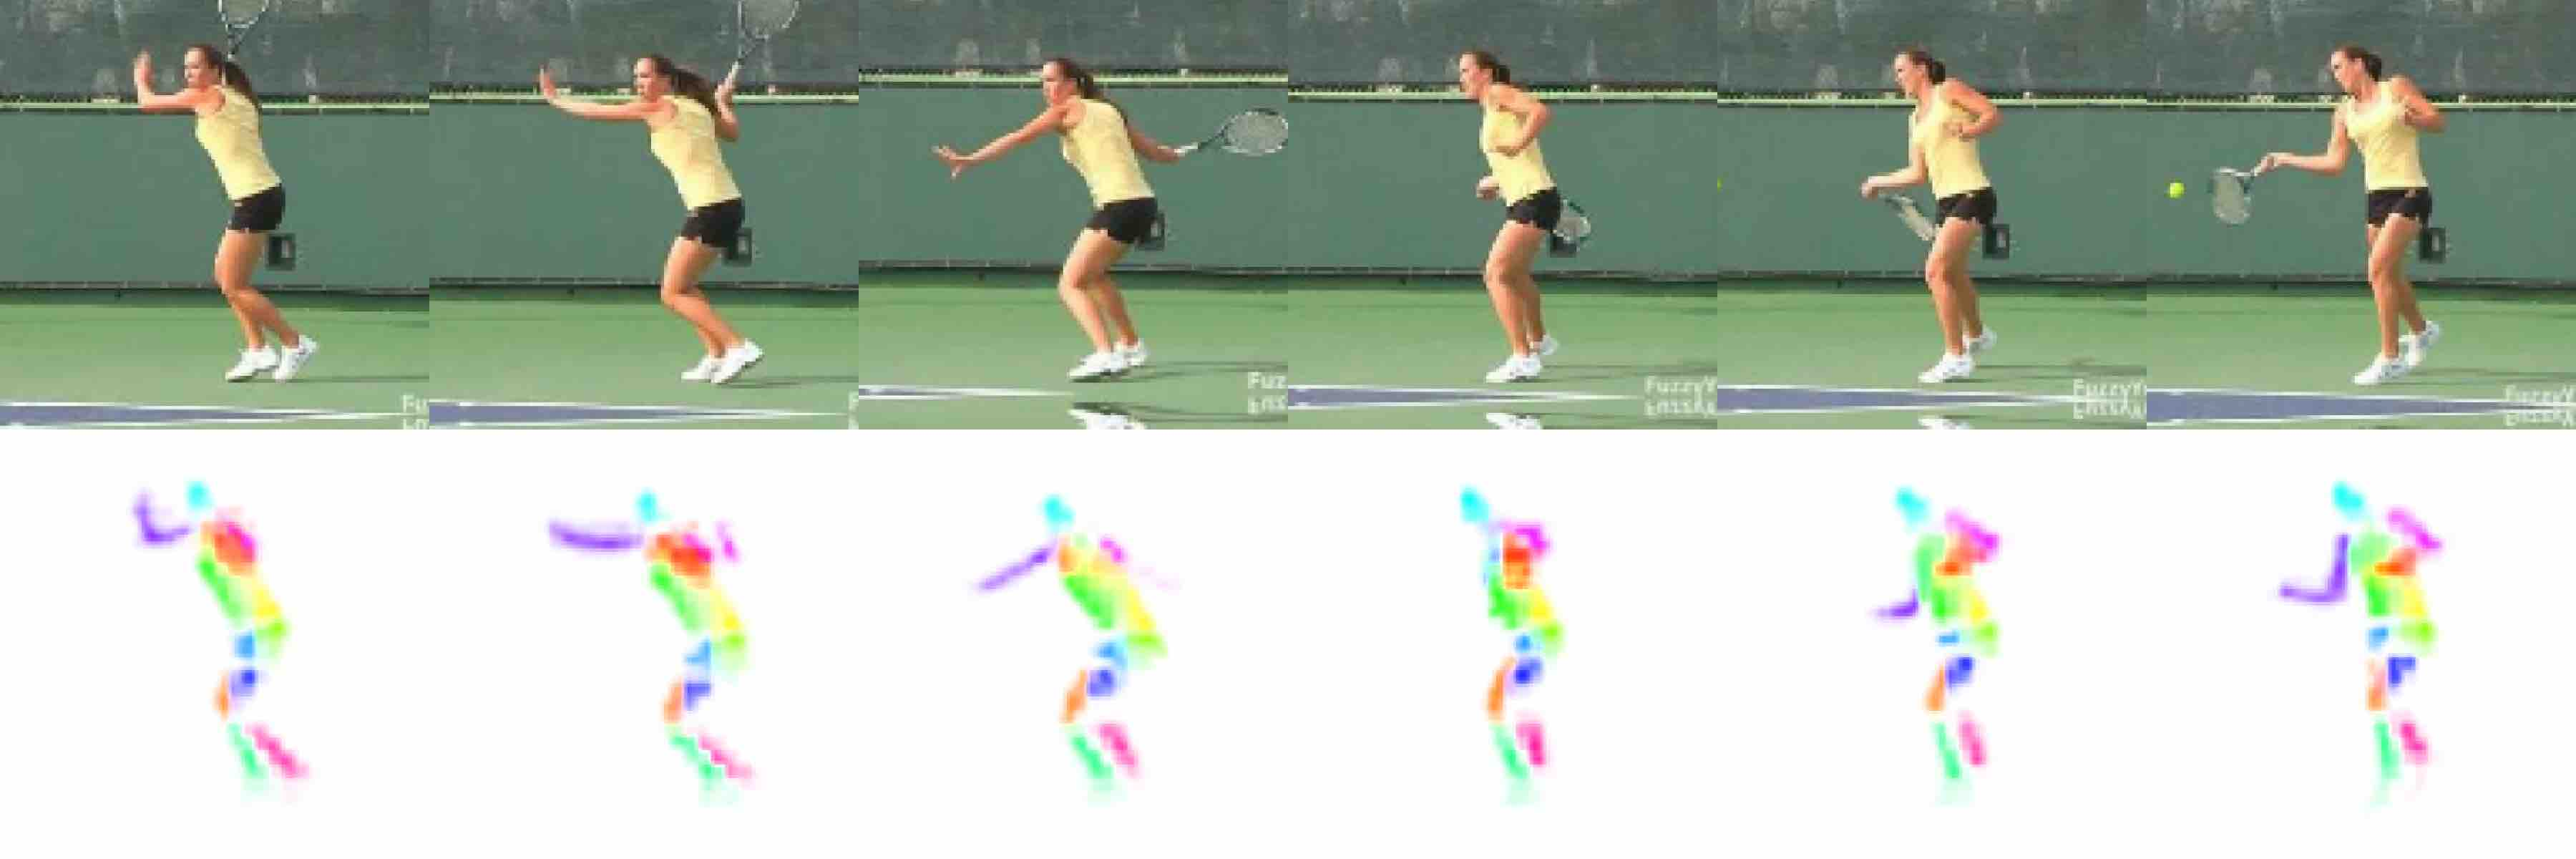
\includegraphics[trim={0cm 0cm 0cm 0cm},clip, width=1.\linewidth]{fig/shape_tennis}\caption{}
	\label{fig:shape_tennis}
	\end{subfigure}
	%\begin{subfigure}{0.5\textwidth}
	%\centering
	%\includegraphics[trim={0cm 0cm 0cm 0cm},clip, width=1.\linewidth]{mat/shape_yoga}\caption{}
	%\label{fig:shape_yoga}
	%\end{subfigure}
	\caption{Learned shape representation on Penn Action. For visualization, 13 of 16 part activation maps are plotted in one image. (a) Different instances, showing intra-class consistency and (b) video sequence, showing consistency and smoothness under motion, although each frame is processed individually.}
	\label{fig:shape}
\end{figure}

\section{Shape Learning}
	% SHOW DISCOVERY
	\begin{figure}[htp]
		\centering
		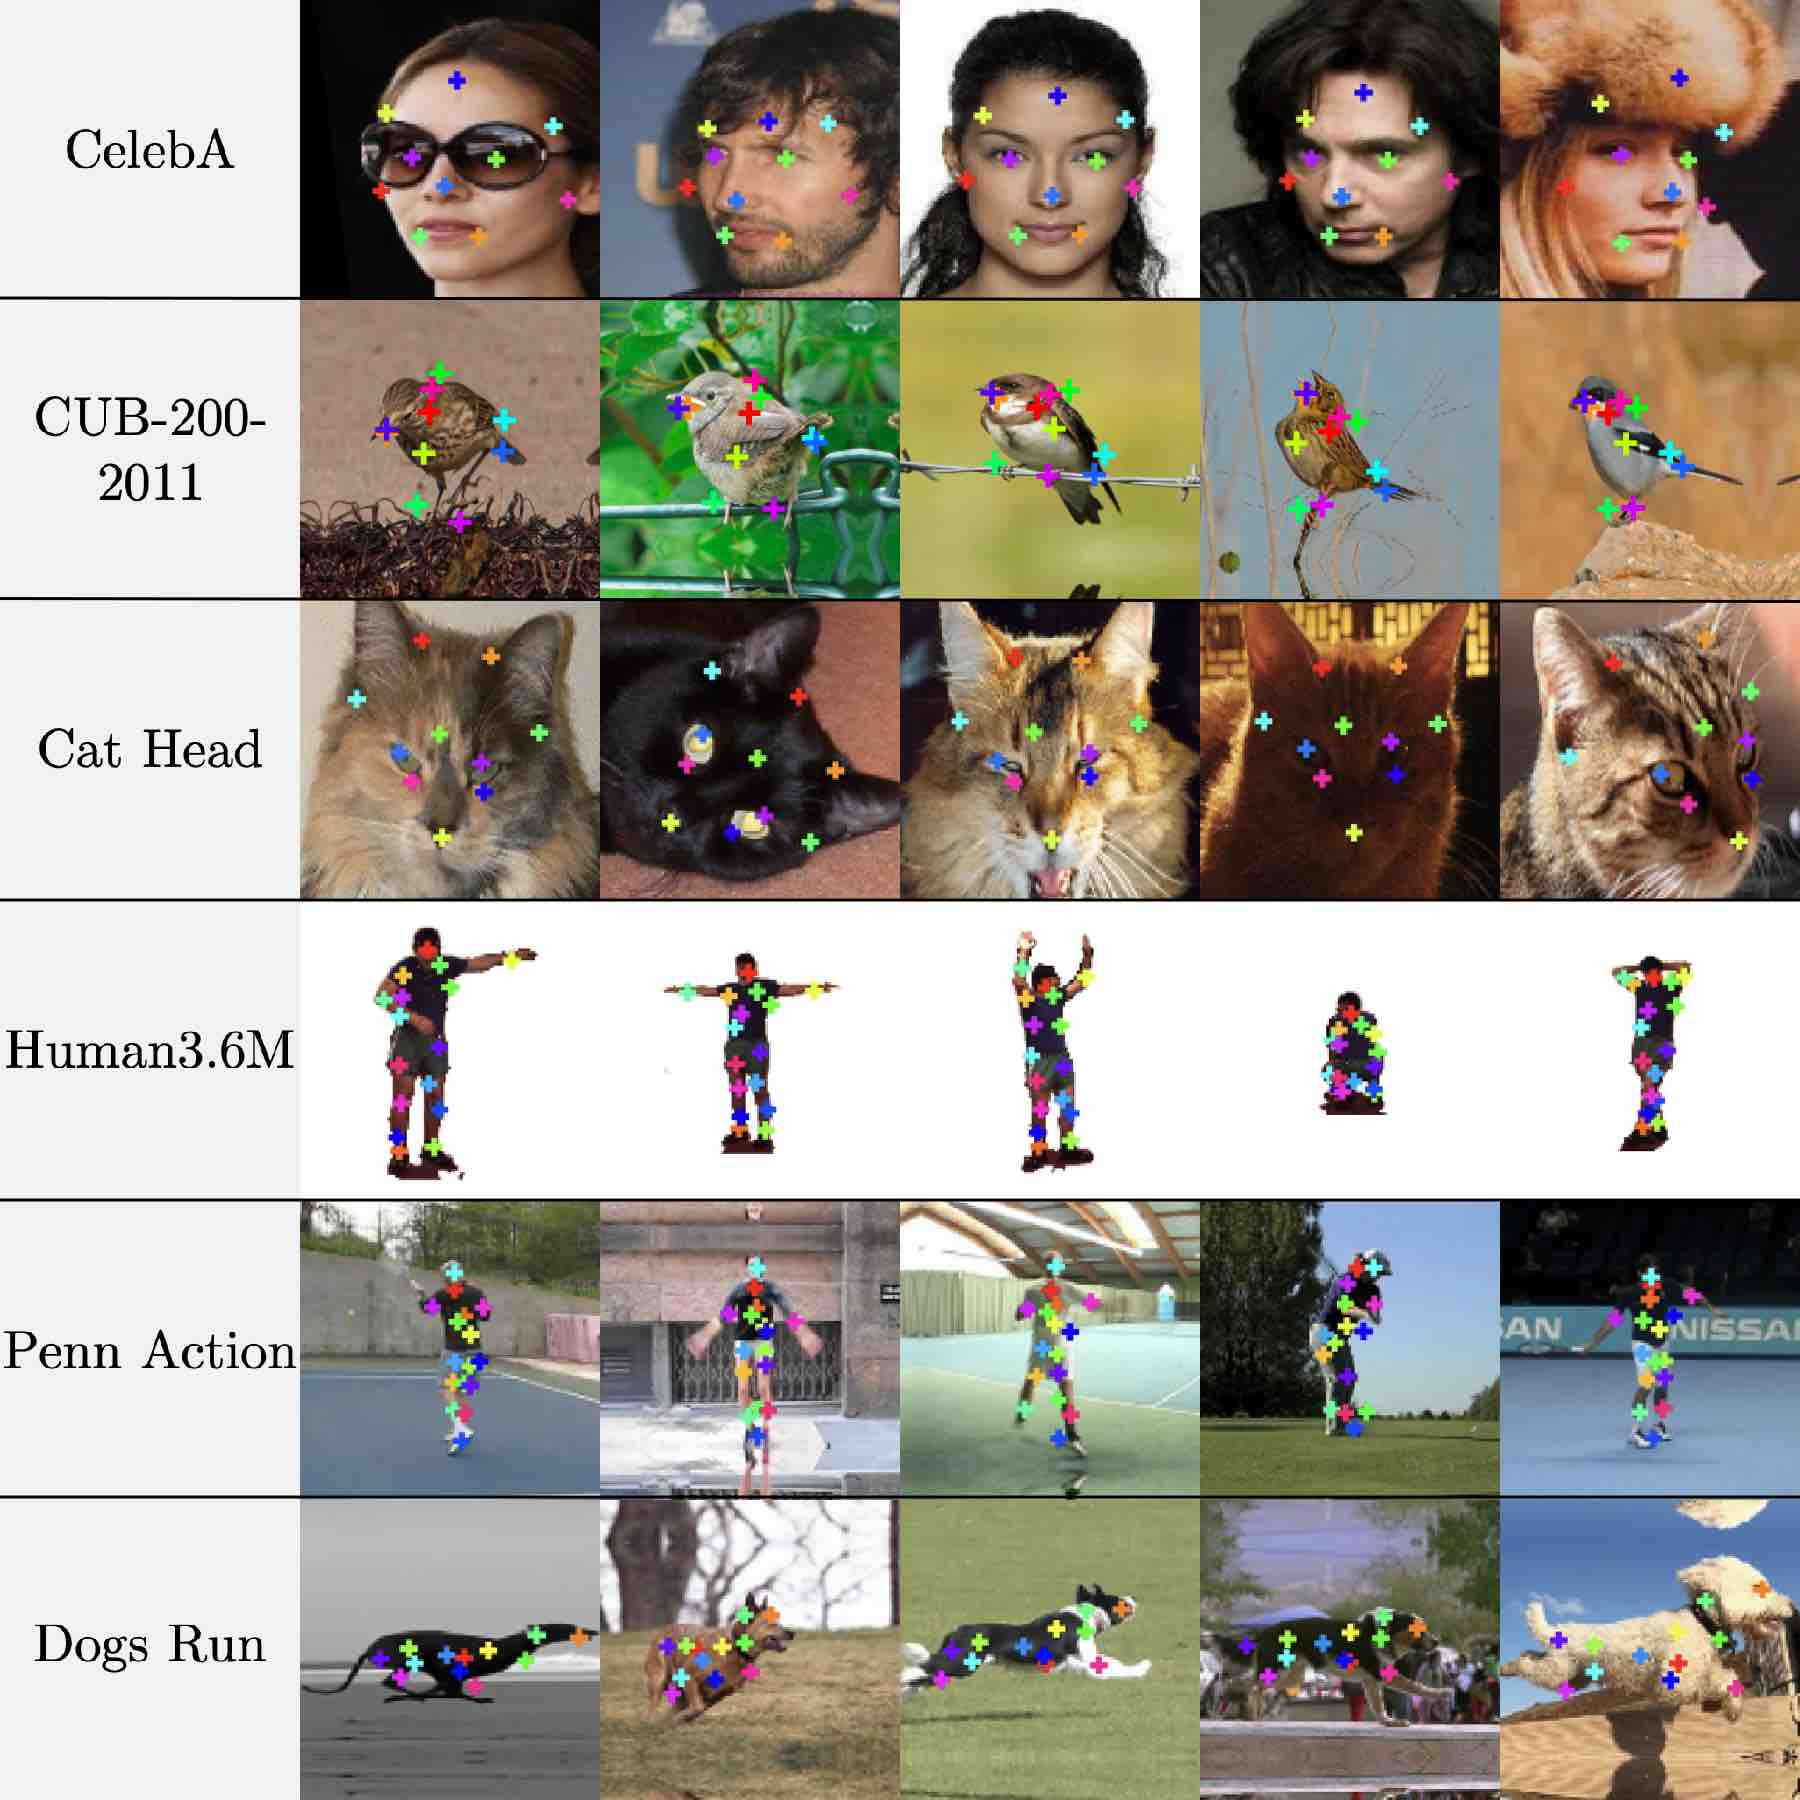
\includegraphics[trim={0cm 0cm 0cm 0cm},clip, width=.6\linewidth]{fig/kp_mania}
		\caption{{Unsupervised discovery of landmarks on diverse object classes such as human or cat faces and birds and for highly articulated human bodies and running dogs.}}
		%(from CelebA, CUB-200-2011 and Cat Head)
		% and on articulated objects such as human bodies and running dogs.}}
		%(from Human3.6M (no background),  Penn Action (real world conditions) and Dogs Run).}}
		\label{fig:kp_mania}
	\end{figure}
	\begin{figure}[htp]
		\centering
		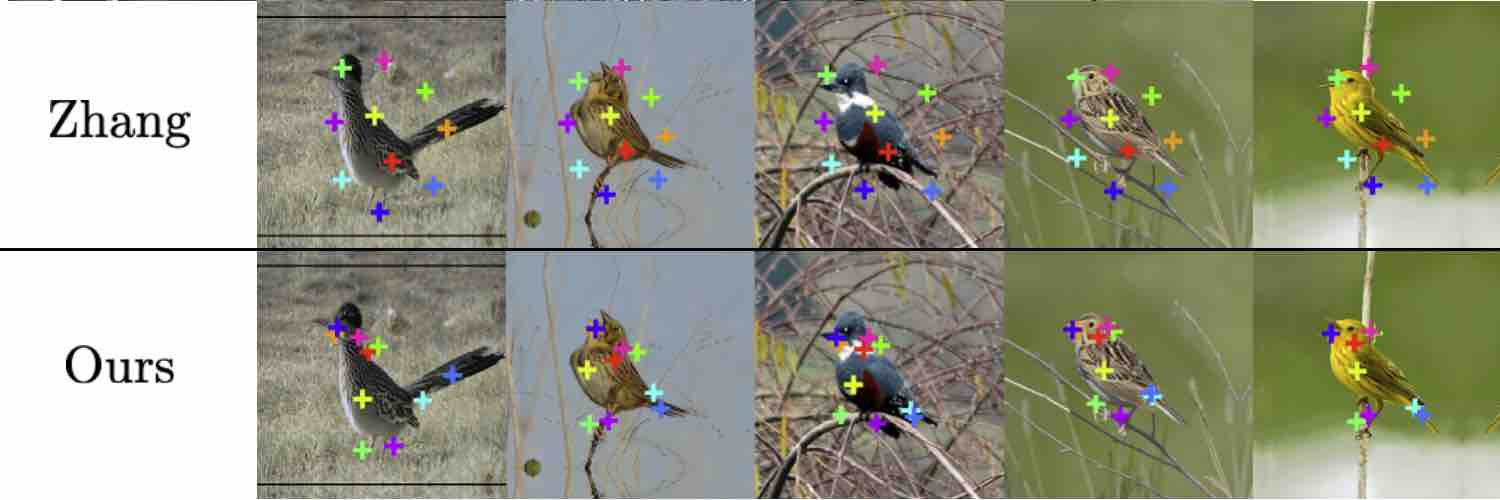
\includegraphics[trim={0cm 0cm 0cm 0cm},clip, width=.7\linewidth]{fig/birds1x3}
		\caption{Comparing discovered keypoints against \cite{zhang18} on CUB-200-2011. We improve on object coverage and landmark consistency. Note our flexible part placement compared to a rather rigid placement of \cite{zhang18} due to their part separation bias.}
		\label{fig:compare}
	\end{figure}
	% STATIC DATASETS: CELEBA, CATS, BIRDS
	% \begin{table}[t]
		% \caption{{Comparison with other unsupervised methods for annotated landmark prediction on the Cat Head, MAFL (subset of CelebA), and CUB-200-2011 testing sets. The
		% error is given in \% of the inter-ocular distance for Cat Head and MAFL and in \% of the edge length of the image for CUB-200-2011.}}
		% \label{tab:static}
		% \centering
		% \begin{tabular}{l|ccccc}
		% \hline
		% Dataset & Cat Head &  & MAFL & & CUB\\
		  % \# Landmarks &10 & 20  & 10 & 30 &10  \\
		  % \hline
		 % Thewlis \cite{thewlis17}
		 % & 26.76 & 26.94 & 6.32 & 5.76 & -  \\
		 % Jakab \cite{jakab18}
		 % & - & - & 4.69 & \textbf{3.08} & - \\
		 % Zhang \cite{zhang18}
		 % & 15.35 & 14.84 & 3.46 & 3.15 & 5.36 \\
		  % Ours & \textbf{9.88}  & \textbf{9.30} & \textbf{3.24} & 3.11 & \textbf{3.91}  \\ \hline  % image length is 600: 32.15 , 23.51
		% \end{tabular}
	% \end{table}
	\begin{table}[t]
		\caption{{Error of unsupervised methods for landmark prediction on the Cat Head, MAFL (subset of CelebA), and CUB-200-2011 testing sets.
		%For Cat Head and MAFL we report error in \% of inter-ocular distance, for CUB-200-2011 it is \% of edge length.
		The	error is in \% of inter-ocular distance for Cat Head and MAFL and in \% of edge length of the image for CUB-200-2011.}}
		\label{tab:static}
		\centering
		\begin{tabular}{l|cccc}
		\hline
		Dataset & Cat Head &  & MAFL & CUB\\
		  \# Landmarks &10 & 20  & 10 &10  \\
		  \hline
		 Thewlis \cite{thewlis17}
		 & 26.76 & 26.94 & 6.32  & -  \\
		 Jakab \cite{jakab18}
		 & - & - & 4.69 & - \\
		 Zhang \cite{zhang18}
		 & 15.35 & 14.84 & 3.46 & 5.36 \\
		  Ours & \textbf{9.88}  & \textbf{9.30} & \textbf{3.24} & \textbf{3.91}  \\ \hline  % image length is 600: 32.15 , 23.51
		\end{tabular}
	\end{table}

	Fig. \ref{fig:shape} visualizes the learned shape representation.
	To quantitatively evaluate the shape estimation, we measure how well groundtruth landmarks (only during testing) are predicted from it.
	The part means $\mu[\sigma_i(x)]$ \todo{make compatible with method} serve as our landmark estimates and we measure the error when linearly regressing the human-annotated groundtruth landmarks from our estimates.
	For this, we follow the protocol of Thewlis \etal \cite{thewlis17}, fixing the network weights after training the model, extracting unsupervised landmarks and training a single linear layer without bias.
	The performance is quantified on a test set by the mean error and the percentage of correct landmarks (PCK).
	We extensively evaluate our model on a diverse set of datasets, each with specific challenges. An overview over the challenges implied by each dataset is given in Tab. \ref{tab:challenges}.
	On all datasets we outperform the state-of-the-art by a significant margin.


	\subsection{Landmark Discovery}
		On the object classes of human faces, cat faces, and birds (datasets CelebA, Cat Head, and CUB-200-2011) our model predicts landmarks consistently across different instances, cf. Fig. \ref{fig:kp_mania}.
		Tab. \ref{tab:static} compares against the state-of-the-art. Due to different breeds and species the Cat Head, CUB-200-2011 exhibit large variations between instances. Especially on these challenging datasets we outperform competing methods by a large margin.
		Fig. \ref{fig:compare} also provides a direct visual comparison to \cite{zhang18} on CUB-200-2011. It becomes evident that our predicted landmarks track the object much more closely. In contrast, \cite{zhang18} have learned a slightly deformable, but still rather rigid grid.
		This is due to their separation constraint, which forces landmarks to be mutually distant. We do not need such a problematic bias in our approach, since the localized, part-based representation and reconstruction guides the shape learning and captures the object and its articulations more closely.

		% BBC POSE Results
		\begin{table}[t]
			\caption{{
			Performance of landmark prediction on BBC Pose test set. As upper bound, we also report the performance of supervised methods.
			%Comparing against supervised and unsupervised methods for annotated landmark prediction on the BBC Pose testing set.
			The metric is \% of points within 6 pixels of groundtruth location. %Note that Jakab et al. are using a 50-landmarks, while we only use a 30 landmarks as input for the regression.
			}}
			\label{tab:bbcpose}
			\centering
			\begin{tabular}{ll|cr}
			\hline
			BBC Pose &   &    { Accuracy}  \\
			 \hline
			supervised & Charles \cite{charles13bbcpose} &
			   79.9\%  \\ % 79.90
			 & Pfister \cite{pfister15flowingconv}  &
			  88.0\%  \\ \hline % 88.01
			unsupervised &Jakab \cite{jakab18} &
			 68.4\%  \\  % 68.44
			  &Ours &  \textbf{74.5}\% \\
			% test pck = 0.7484605918670523
			% test pck_per_kp = [0.9633621  0.6627155  0.76508623 0.54956895 0.6928879  0.76616377   0.83943963]
			\hline
			\end{tabular}
		\end{table}
		% HUMAN3.6M Results
		\begin{table}[t]
			\caption{{Comparing against supervised, semi-supervised and unsupervised methods for landmark prediction on the Human3.6M test set. The
			error is in \% of the edge length of the image. All methods predict 16 landmarks.
			}}
			\label{tab:human}
			\centering
			\begin{tabular}{ll|cr}
			\hline
			 Human3.6M   & &  { Error w.r.t. image size}  \\
			 \hline
			 supervised & Newell \cite{newell16hourglass}
			  &2.16  \\  \hline
			 semi-supervised & Zhang \cite{zhang18}
			  & 4.14  \\ \hline
			 unsupervised & Thewlis \cite{thewlis17}
			 & 7.51  \\
			  & Zhang \cite{zhang18}
				& 4.91 \\
			  & Ours& \textbf{2.79} \\
			\hline
			\end{tabular}
		\end{table}

		\subsubsection{Human Faces}
		\todo{make figures}
		\subsubsection{Human Bodies}
		Human, Olympic, Penn
		\subsubsection{Animal Faces/Bodies}
		Dogs, Cats, Birds
		\subsubsection{Composite Objects/Scenes}
		What is an object? What is a scene?
		compositional nature of reality
		Bird on twig object? Bird can also fly, but neural networks learn by correlation in data (-> ref to these ''failure modes''
		Dancing pair as object.
		\subsubsection{Object/Background Separation}
			Complexly cluttered background is actually favorable for the method. Correlations of object with background will belong to object.
		\subsubsection{Object Articulation}
			Object articulation makes consistent landmark discovery challenging.
			Fig. \ref{fig:kp_mania} shows that our model exhibits strong landmark consistency under articulation and covers the full human body meaningfully.
			Even fine-grained parts such as the arms are tracked across heavy body articulations, which are frequent in the Human3.6M and Penn Action datasets.
			Despite further complications such as viewpoint variations or blurred limbs our model can detect landmarks on Penn Action of similar quality as in the more constrained Human3.6M dataset.
			Additionally, complex background clutter as in BBC Pose and Penn Action, does not hinder finding the object.
			Experiments on the Dogs Run dataset underlines that even completely dissimilar dog breeds can be related via semantic parts.
			Tab. \ref{tab:bbcpose} and Tab. \ref{tab:human} summarize the quantitative evaluations: we outperform other unsupervised and semi-supervised methods by a large margin on both datasets.
			On Human3.6M, our approach achieves a large performance gain even compared to methods that utilize optical flow supervision.
			On BBC Pose, we outperform \cite{jakab18} by $6.1\%$, reducing the performance gap to supervised methods significantly.
	\subsection{Effect of Transformations}
		\note{in this section: effect of transformations on learning, disentangling}
		\note{effectively connecting samples from the dataset, spreading the}
		\subsubsection{Parity}
		birds parity
		salsa parity
		\subsubsection{Rotation, Scaling, Translation}
			on Cats -> black cats different set of KP than rest -> connect these samples via transformation to reach intra-class consistency
		\subsubsection{Mimicking Appearance}
		Color, Contrast, Hue
		\subsection{Natural Changes}
		Video data: Penn, Own
\section{Disentangling Generative Factors}

	% POSE APPEARANCE SWAP
	\begin{figure}[t]
		\centering
		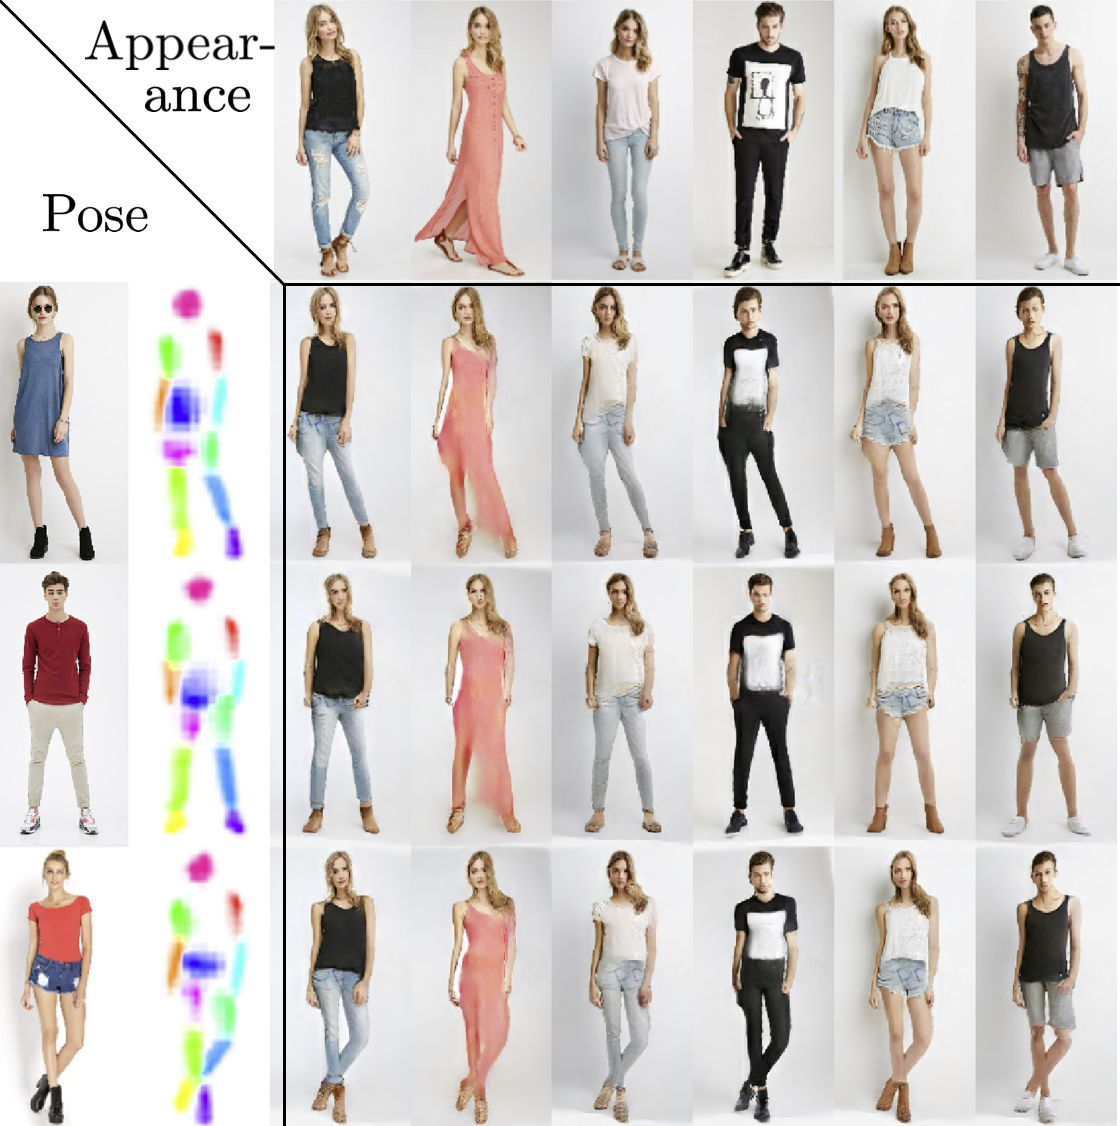
\includegraphics[trim={0cm 0cm 0cm 0cm},clip, width=.7\linewidth]{fig/swappy}
		\caption{Transferring shape and appearance on Deep Fashion. Without annotation the model estimates shape, 2nd column. Target appearance is extracted from images in top row to synthesize images. Note that we trained without image pairs only using synthetic transformations.
		%for training we had no image pairs but only synthetic transformations.
		%without being explicitly trained for this task.
		All images are from test set.}
		\label{fig:allswaps}
	\end{figure}

	\begin{table}
		\centering
		\caption{Mean average precision (mAP) and rank-n accuracy for person re-identification on synthesized images after performing shape/appearance swap. Input images from Deep Fashion test set. Note \cite{esser18} is supervised w.r.t. shape.}
		\label{tab:reid}
		\begin{tabular}{l|cccr}
			\hline
			& mAP & rank-1 & rank-5 & rank-10 \\ \hline
			VU-Net \cite{esser18} & 88.7\% & 87.5\% & {98.7}\% & {99.5}\% \\
			Ours & {90.3}\% & {89.4}\% &{98.2}\% & {99.2}\% \\ \hline
		\end{tabular}
	\end{table}
	\begin{table}
		\centering
		\caption{Percentage of Correct Keypoints (PCK) for pose estimation on shape/appearance swapped generations.\;$\alpha$ is pixel distance divided by image diagonal. Note that \cite{esser18} serves as upper bound, as it uses the groundtruth shape estimates.}
		%shape supervision.}
		\label{tab:pose}
		\begin{tabular}{l|cccr}
			\hline
			$\alpha$ & $2.5\%$ &  $5\%$ & $7.5\%$ & $10\%$ \\ \hline
			VU-Net \cite{esser18} & {95.2}\% & {98.4}\% & {98.9}\% & {99.1}\% \\
			Ours & 85.6\% & 94.2\% &96.5\% & 97.4\% \\ \hline
		\end{tabular}
	\end{table}

	% BBC THUMB

	\begin{figure}[t]
		\centering
		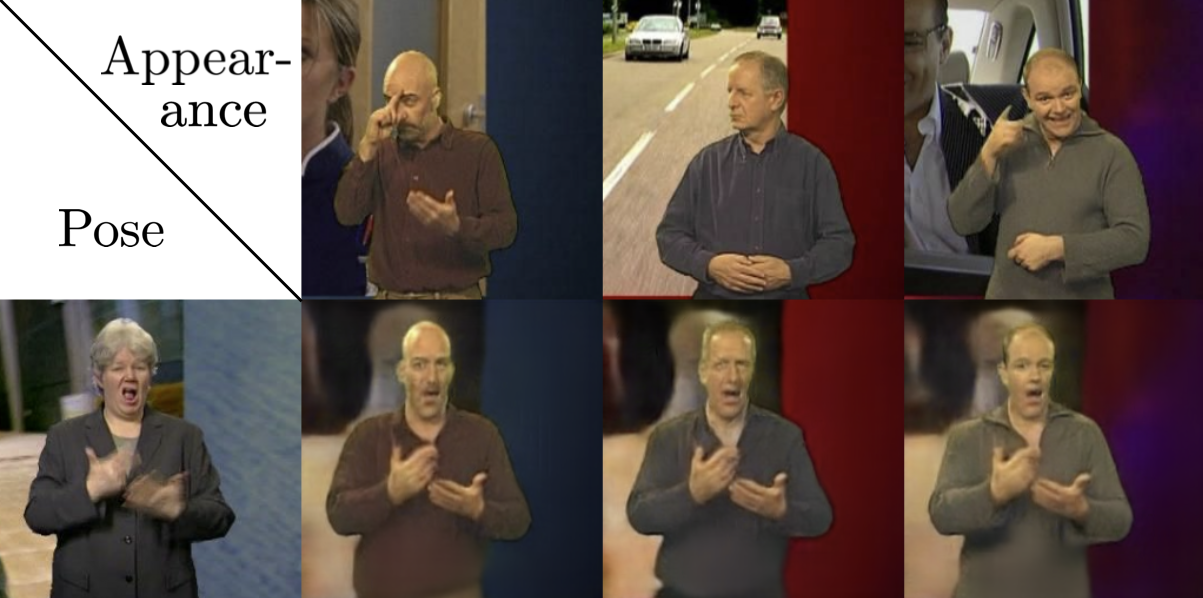
\includegraphics[trim={0cm 0cm 0cm 0cm},clip, width=.7\linewidth]{fig/bbcthumb}
		\caption{Video-to-video translation on BBC Pose. Top-row: target appearances, left: target pose.
		%The target appearances are from the train set, while the target pose is from the test set.
		Note that even fine details in shape are accurately captured. See supplementary for videos.}
		\label{fig:bbcthumb}
	\end{figure}

	Disentangled representations of object shape and appearance allow to alter both properties individually to synthesize new images. The ability to flexibly control the generator allows, for instance, to change the pose of a person or their clothing. In contrast to previous work \cite{esser18, denton17disvideo, ma17poseguided, ma17disperson, debem18dgpose, jakab18},
	we achieve this ability without requiring supervision \textit{and} using a flexible part-based model instead of a holistic representation. This allows to explicitly control the parts of an object that are to be altered. We quantitatively compare against \emph{supervised} state-of-the-art disentangled synthesis of human figures. Also we qualitatively evaluate our model on unsupervised synthesis of still images, video-to-video translation, and local editing for appearance transfer.


	t-SNE of Shape Representation
	t-SNE of Appearance Representation


	\subsection{Disentangling Pose and Appearance}


	On Deep Fashion \cite{liu16deepfashion, liu16deepfashionwild}, a benchmark dataset for supervised disentangling methods, the task is to separate person ID (appearance) from body pose (shape) and then synthesize new images for previously unseen persons from the test set in eight different poses. We randomly sample the target pose and appearance conditioning from the test set. Fig. \ref{fig:allswaps} shows qualitative results.
	We quantitatively compare against supervised state-of-the-art disentangling \cite{esser18} by evaluating \emph{i)} invariance of appearance against variation in shape by the re-identification error and \emph{ii)} invariance of shape against variation in appearance by the distance in pose between generated and pose target image.

	\subsubsection{ReID}
	\begin{itemize}
		\item t-SNE of IDs
		\item Own, Other (stronger statement)
	\end{itemize}
	To evaluate appearance we fine-tune an ImageNet-pretrained \cite{russakovsky15imagenet} Inception-Net \cite{szegedy15inception} with a re-identification (ReID) algorithm \cite{xiao17reidjoint} via a triplet loss \cite{hermans17reidtriplet} to the Deep Fashion training set.
	On the generated images we evaluate the standard metrics for ReID, mean average precision (mAP) and rank-1, -5, and -10 accuracy in Tab. \ref{tab:reid}.
	Although our approach is unsupervised it is competitive compared to the supervised VU-Net \cite{esser18}.


	\subsubsection{Pose}
	To evaluate shape, we extract keypoints using the pose estimator \cite{cao17affinityfield}. Tab. \ref{tab:pose} reports the difference between generated and pose target in percentage of correct keypoints (PCK). As would be expected, VU-Net performs better, since it is trained with exactly the keypoints of \cite{cao17affinityfield}. Still our approach achieves an impressive PCK without supervision underlining the disentanglement of appearance and shape.

	\begin{itemize}
		\item PCK Curve
	\end{itemize}

	\subsection{Factorizing into Parts}
	% PART SWAPS
	\begin{figure}[t]
		\begin{subfigure}{0.24\linewidth}
		\centering
		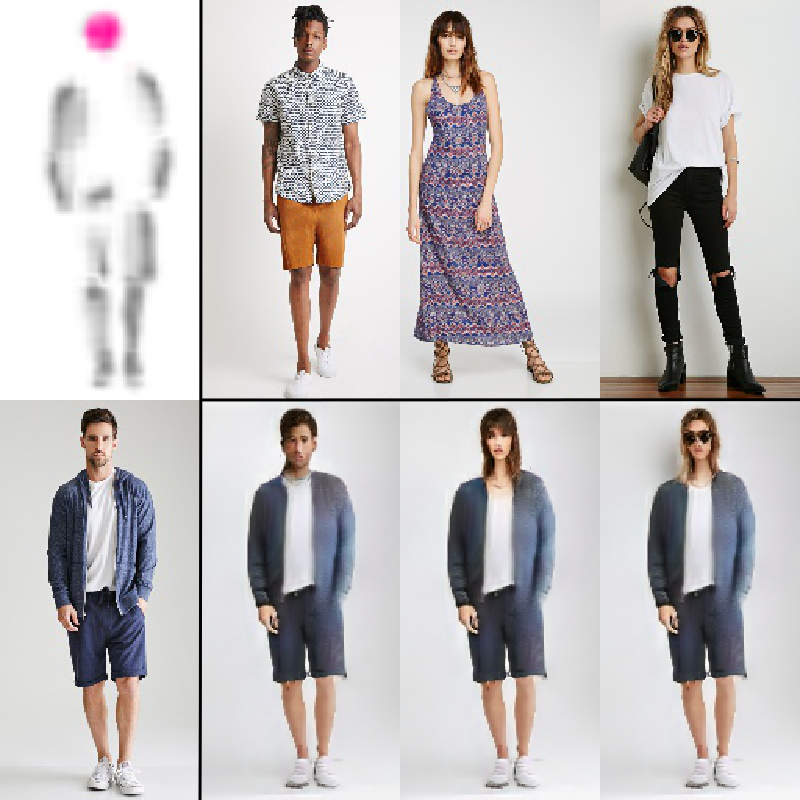
\includegraphics[trim={0cm 0cm 0cm 0cm},clip, width=1.\linewidth]{fig/part_head}\caption{}
		\label{fig:part3_00}
		\end{subfigure}
		\begin{subfigure}{0.24\linewidth}
		\centering
		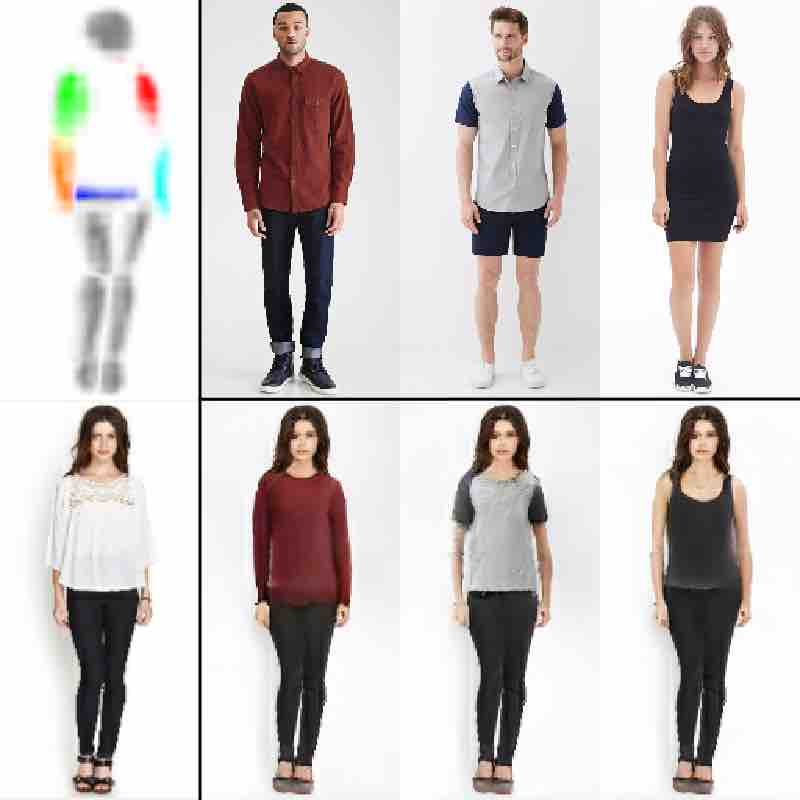
\includegraphics[trim={0cm 0cm 0cm 0cm},clip, width=1.\linewidth]{fig/part_body}\caption{}
		\label{fig:part3_11}
		\end{subfigure}
		\begin{subfigure}{0.24\linewidth}
		\centering
		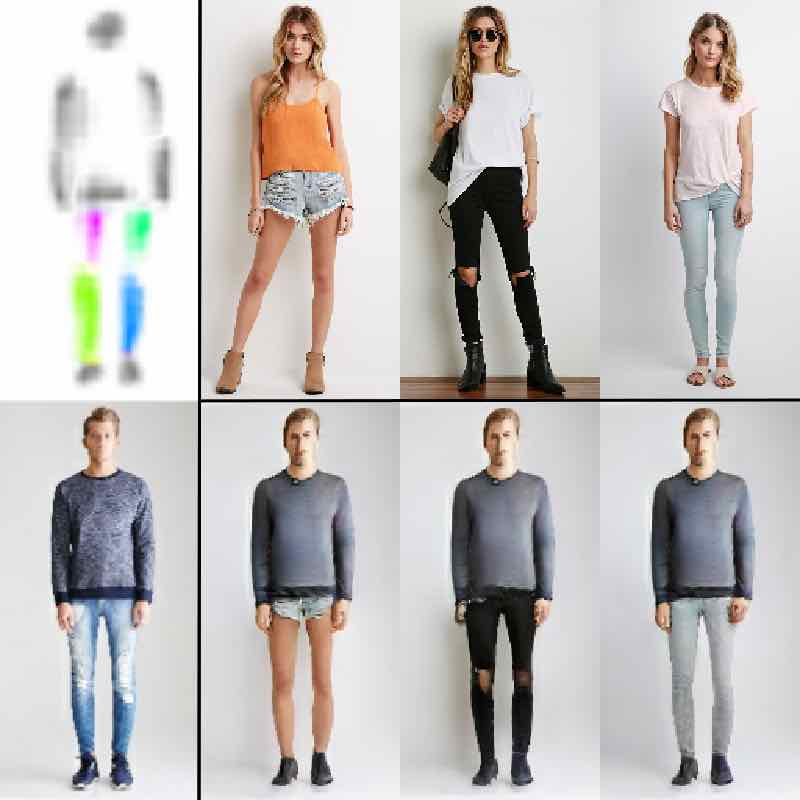
\includegraphics[trim={0cm 0cm 0cm 0cm},clip, width=1.\linewidth]{fig/part_legs}\caption{}
		\label{fig:part3_21}
		\end{subfigure}
		\begin{subfigure}{0.24\linewidth}
		\centering
		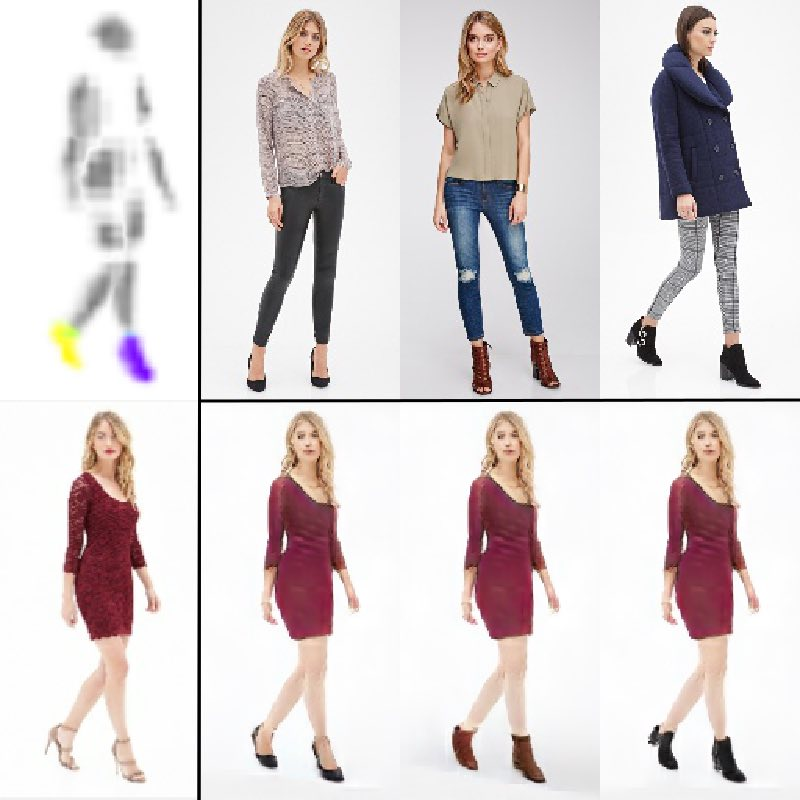
\includegraphics[trim={0cm 0cm 0cm 0cm},clip, width=1.\linewidth]{fig/part_shoe}\caption{}
		\label{fig:part3_30}
		\end{subfigure}
		\caption{Swapping part appearance on Deep Fashion. Appearances can be exchanged for parts individually and without altering shape. We show part-wise swaps for (a) head (b) torso (c) legs, (d) shoes. All images are from the test set.}
		\label{fig:partswaps}
	\end{figure}
	\begin{itemize}
		\item Own Dataset: Move KP
		\item DeepFashion: exchange parts
	\end{itemize}

\section{Follow-Up}
	\begin{itemize}
		\item make generative:(KP distribution estimation, variational features).
		\item make video generation possible (RNN on KP vector).
		\item better transformations -> appearance locally (around parts changed), appearance changed perceptually -> style transfer
	\end{itemize}






	% \chapter{Discussion}


\chapter{Conclusion}

\section{Final Thoughts}\label{sec:finalthoughts}

	\note{specifying factors in advance good
	-> need model-based approach (for counterfactual)
	%
	% make model as good as we can implementing as many assumptions as we can and only leave the rest to powerful model
	(humans also have brain structure and reasoning structure genetic) in general orient after human good
	%
	need disentangling generative factors for imagination (\ie synthesis)
	for manipulating factors mentally
	%
	causality will be shed light on many endeavours in artificial intelligence not only disentangling}

	% summary
	We have presented an unsupervised approach to learning the compositional part structure of objects by disentangling geometric shape from visual appearance. We derive invariance and equivariance constraints that enable a generative framework to discover consistent landmarks without requiring a prior assumptions on landmark layout. Experiments show that our approach significantly improves upon previous unsupervised methods.
 	% context of causality
	Disentangling shape and appearance has been presented in the broader context of learning the causal structure of the world through images. The insights from the causal literature let us rethink the role of priors, models and data and give a direction for future work.
	% final metaphor/ joke/ twist
	% broader context: build intelligent machines. images to imagination.
	% thanks
	\note{next step entangling further, to disentangle further}
	\note{rethink disentanglement, \eg parts have dependencies, but exactly by modelling those dependencies reach disentanglement, similar to appearance conditioning in order to extract shape. look for bengio talk}

	Throughout this work we alluded to two themes: \emph{i)} improving models with realistic constraints and assumptions \emph{ii)} extracting value from richer data, \ie interventional and temporal data.
	For our task of disentangling shape and appearance of objects these themes translated into \emph{i)} better modelling of the synthesis side in the analysis-by-synthesis framework and \emph{ii)} utilizing image transformations \wrt which to capture invariant and equivariant factors.


\section{Future Work}\label{sec:futurework}

	% \begin{itemize}
		% \item make generative:(KP distribution estimation, variational features).
		% \item make video generation possible (RNN on KP vector).
		% \item better transformations -> appearance locally (around parts changed), appearance changed perceptually -> style transfer
		% \item local appearance change (as TPS)
	% \end{itemize}

	With regards to these two themes there are obvious improvements to be made:


	\emph{i)} On the modelling side our method models the interplay between shape and appearance of a composite object, but in a prototypical manner. Realistic graphical simulation - as long as it is fully differentiable - such as used in ~\cite{kulkarni15dcign, tieleman14thesis} would impose tighter constraints onto how the factors generate the image.
	\note{bengio: disentanglement by modelling entanglement, modelling or learning the physical laws on how the factors interact. Change in shape changes appearance (in image) \eg zebra stripes.}

	% temporal data
	\emph{ii)} On the data side a next step could be to model video data in the exact temporal sequence, not only on a frame-by-frame level (cf. Sec.~\ref{sec:videotovideo}). To do this, the temporal changes of shape would be necessary to be modelled. For this it could prove useful to make our model generative. Generating appearance features could be implemented with standard variational features~\cite{kingma13vae}. Generating shape for temporal sequences could use some type of recurrent architecture.
	% could make model generative for video sequences, in general generative side is easy to supplement with making features variational, the shape condiditoning could be sampled from, after learning, by estimating the distribution of landmarks and their correlation matrix for the training dataset
	% interventional data
	We also repeatedly stressed the importance of the image transformations. For disentangling they are the necessary condition. The better the transformations separate variation in the to-be-disentangled-factors, the better disentangled will these factors be. Video data are the best source of shape transformations, for appearance however, the global contrast, brightness and hue transformations are neither natural nor complete of any type of appearance transform. Usually patterns and texture are considered as appearance, hence, for completeness they should also be transformed. This could be tried with a soft form of style alteration via style transfer~\cite{gatys15neuralstyle}. In addition to extending appearance transformations to a higher level, one can also make them more local, this would further encourage the factorization into local parts.




	% \section{Contributions I}
	\textbf{Hypothesis}: learning shape requires abstracting away appearance -> hence disentangling
	% \textbf{Hypothesis \emph{ii)}}: learning disentanglement from data is fundamentally constrained. disentangling without supervision impossible from pure data and without explicit model
	% need to interact with the world, need to change, need to model physical reality -> image transformations, analyis-by-synthesis
	\begin{itemize}
		\item validate and evaluate method developed by Lorenz \etal\ 2018 for disentangling
		\item overview over state-of-the-art disentangling, analysis of future directions
		\item explain method in context to these
		\item evaluate unsupervised shape learning:
			\begin{itemize}
				\item human faces, bodies (CelebA, Human3.6M)
				\item animal faces, bodies (cats, dogs, birds)
				\item composite objects (dancing pair)
			\end{itemize}
		\item make own video dataset
			\begin{itemize}
				\item for disentangling human pose and appearance (heidelbergpose)
				\item for articulated animal video (dogs)
				\item for composite object (pair dancing salsa)
			\end{itemize}
		\item ablation study (reconstruction, equivariance loss, transformations)
		\item study: effect of image transformations
		\item qualitative comparison to non-disentangling composite shape learning (Zhang)
		\item evaluating disentanglement
			\begin{itemize}
				\item reID
				\item pose estimation
			\end{itemize}
	\end{itemize}
	result: soa in shape learning, (first) unsupervised disentangling of articulated shape and appearance
\newpage
\section{Contributions II}
	\textbf{Hypothesis}: learning object shape efficiently requires a composite explanation in terms of equivariant parts.
	\begin{itemize}
		\item develop and analyze method for learning object shape
		\item performance analysis of:
			\begin{itemize}
				\item hierarchy of parts
				\item number of keypoints
				\item local loss weighting
				\item feature aggregation (1/1+..)
				\item part shapes (qualitatively Penn Action)
			\end{itemize}
		\item make dataset (heidelbergpose)
		\item compare against holistic representation (Jakab) on BBCPose quantitatively
		\item generative results on human poses, faces (KTH, CelebA, Human)
		\item add part-wise adversarial task (BBCPose, DeepFashion)
		\item part-wise swapping, moving parts independently (DF, and own data)
	\end{itemize}
	result: state-of-the-art in unsupervised shape learning, learning part regions unsupervised, manipulating generation part-wise possible

	\part{Appendix}
	\begin{appendix}
	\chapter{Datasets}
	\textbf{CelebA} \cite{liu15facewild} contains ca. 200k celebrity faces of 10k identities.
We resize all images to $128\times 128$ and exclude the training and test set of the MAFL subset, following \cite{thewlis17}.
As  \cite{thewlis17, zhang18}, we train the regression (to 5 ground truth landmarks) on the MAFL training set (19k images) and test on the MAFL test set (1k images).

\textbf{Cat Head} \cite{zhang08cathead}  has nearly 9k images of cat heads.
We use the train-test split of \cite{zhang18} for training (7,747 images) and testing (1,257 images).
We regress 5 of the 7 (same as \cite{zhang18}) annotated landmarks.
The images are cropped by bounding boxes constructed around the mean of the ground truth landmark coordinates and resized to $128\times128$.


\textbf{CUB-200-2011} \cite{wah11birds} comprises ca. 12k images of birds in the wild from 200 bird species.
We excluded bird species of seabirds, roughly cropped using the provided landmarks as bounding box information and resized to $128\times128$.
We aligned the parity with the information about the visibility of the eye landmark.
For comparing with \cite{zhang18} we used their published code.


\textbf{BBC Pose} \cite{charles13bbcpose} contains videos of sign-language signers with varied appearance in front of a changing background. Like \cite{jakab18} we loosely crop around the signers.
The test set includes 1000 frames and the test set signers did not appear in the train set.
For evaluation, as \cite{jakab18}, we utilized the provided evaluation script, which measures the PCK around $d=6$ pixels in the original image resolution.


\textbf{Human3.6M} \cite{ionescu14human36m} features human activity videos.
We adopt the training and evaluation procedure of \cite{zhang18}.
For proper comparison to \cite{zhang18} we also removed the background using the off-the-shelf unsupervised background subtraction method provided in the dataset.


\textbf{Penn Action} \cite{zhang13penn} contains 2326 video sequences of 15 different sports categories.
For this experiment we use 6 categories (tennis serve, tennis forehand, baseball pitch, baseball swing, jumping jacks, golf swing).
We roughly cropped the images around the person, using the provided bounding boxes, then resized to $128\times128$.


\textbf{Dogs Run} is made from dog videos from YouTube totaling in 1250 images under similar conditions as in Penn Action. The dogs are running in one direction in front of varying backgrounds. The 17 different dog breeds exhibit widely varying appearances.


\textbf{Deep Fashion} \cite{liu16deepfashion, liu16deepfashionwild} consists of ca. 53k in-shop clothes images in high-resolution of $256 \times 256$. We selected the images which are showing a full body (all keypoints visible, measured with the pose estimator by \cite{cao17affinityfield}) and used the provided train-test split.
For comparison with Esser \etal \cite{esser18} we used their published code.



	\chapter{Lists}
	\listoffigures
	\listoftables
	\bibliography{lib_new}{}
	% \citestyle{egu}
	% \bibliographystyle{ieee}
	\bibliographystyle{unsrt}
	% \bibliographystyle{plainnat}
	% \setlength{\parindent}{0em}

Erkl\"{a}rung:\par
\vspace{3\baselineskip}
Ich versichere, dass ich diese Arbeit selbstst\"{a}ndig verfasst habe und keine
anderen als die angegebenen Quellen und Hilfsmittel benutzt habe.\par
\vspace{5\baselineskip}
Heidelberg, den (Datum)\hspace{3cm}\dotfill

	\end{appendix}
\end{document}
